\chapter{Analysis}

\section{Introduction}

\subsection{Client Identification}

My Client is Team Cambridge Cycling Club, they run cycling events around Cambridge for any one that wishes to enter. The end user of the project are the members of Team Cambridge so that results can be uploaded soon after an event, as currently only the Racing Secretary can upload results due to the complexity of the current system. The Racing Secretary is Paul Millard currently he uses computers daily for his work, he created the club website, and he maintains the current database that hold the results of each event the club holds. This is carried out on an Acer laptop running Windows Vista 32 bit.

My Client is Team Cambridge Cycling Club, they run cycling events around Cambridge for anyone that wishes to enter. The end users of the project are the members of Team Cambridge so that results can be uploaded soon after an event, as currently only the Racing Secretary can upload results due to the complexity of the existing system. The Racing Secretary is Paul Millard currently he uses computers daily for his work, he created the club website, and he maintains the current database that hold the results of each event the club holds. This is carried out on an Acer laptop running Windows Vista 32 bit.


\subsection{Define the current system}
I was able to interview Paul Millard about the existing system, Paul also was able to provide me with a specification of the existing system outlining how the different systems work. Both are attached in the section appendix.


The current system uses a mix of manual data entry and automatic calculation. Depending on the type of the event held determines the type of calculation that needs to be made, however some of the calculations are used across multiple types of event. The competitions that Team Cambridge members are entered for are Transmedia, Handicap 10, Circuit, Juvenile(if under age 16), Handicap 25  and Hill Climb, once a year Team Cambridge holds an open event currently due to the complexity of the results they are uploaded as a link to a results document. 

Currently the system works as listed below.
\begin{itemize}
	\item Riders attend events and the timekeepers collect the data from the event.
	
	\item The data that timekeepers collect is the name, position, watch time, ride time, emergency
	 telephone number, club, age (only required if under 18), riders signature, event date and event code. Of this data position and watch time are used for calculations only and are not stored in the database, as name, club , age, event date and event code ar recorded in the database.
	 
	\item After the event the Timekeepers give the data to the Racing Secretary.
	
	\item The Racing Secretary enters the name, club, position and watch time in to an Excel spreadsheet.
	
	\item The Excel spreadsheet uses a function to find the ride time by taking the position from the minutes of the watch time.
	
	\item Were an event includes a handicap competition then the following process is performed:
	
	\begin{itemize}
	\item For every Team Cambridge member that competed in the event, Paul finds the best time for the same distance from the existing database, he then enters the data into the spreadsheet.
	
	\item The spreadsheet then uses a lookup function to find the handicap modifier from the lookup table, you can find a copy of this on the last 3 pages of the specification sheet.
	
	\item The modifier is taken from the ride time to find the riders handicap time for that event.
	
	\item The handicap times for all riders are then ordered low to high and points are awarded, the fastest rider is given 20 points, the seconds fastest 19 this continues down to 1 point.
	\end{itemize}
	
	\item Were an event includes a non-handicap competition then the following process is performed
	
	\begin{itemize}
	\item For all Team Cambridge the ride times are ordered low to high.
	
	\item Then points are awarded, the fastest time is given 20 points the second fastest is given 19 this continues down to 1 point.
	\end{itemize}
	
	\item After all the points have been calculated for all competitions affected by the event, the spreadsheet is saved as a .csv file and is uploaded to a database with a web interface.
\end{itemize}

After the event finishes Paul enter the results in to a Microsoft Excel spread sheet, for handicapped competitions the personal best of each rider needs to be looked up and added to the spread sheet. Any calculations that need to be executed are done by the spread sheet and are ordered. The results are then manually added to the current database. A copy of the results are uploaded to the website and the competitions that are effected by the event are updated.

The competitions that Team Cambridge host is shown in the table below and whether they are a handicap competition or non-handicap competition:

\begin{tabular}{|l | l|}
	\hline
	HANDICAP COMPETITIONS & NON-HANDICAP COMPETITIONS \\ \hline
	Circuit Series        & Hill Climb \\ \hline 
	Handicap 10           & Transmedia \\ \hline
	Handicap 25           & Juvenile Series \\ \hline
\end{tabular}

\subsection{Describe the problems}

The current system has lots of manual steps that can cause the process to take a long time, currently it takes on average 2 hours to process and upload one set of results

The current system has manual steps, such as finding the best times and imputing or creating a new rider, that cause the process to take a long time. Currently it takes on average 2 hours to process and upload one set of results.

The steps that could be automated are the detection of a new rider, calling of a riders personal best, any calculations and sorting of the times and uploading data to the database

The database has been changed to accommodate the way the results are displayed on the website. Following these changes  however, unnecessary parts were not removed.

The steps that could be automated are the detection and creation of a new rider and finding a riders personal best time; all of the calculation mentioned so far can be fully automatic, uploading the results to the website can also be automated.



\subsection{Section appendix}


The Specification supplied by Paul Millard.

\begin{figure}[H]
    
\includegraphics[width=\textwidth]{./TeamCambridgeSpec/page1.pdf}
\end{figure}

\begin{figure}[H]
    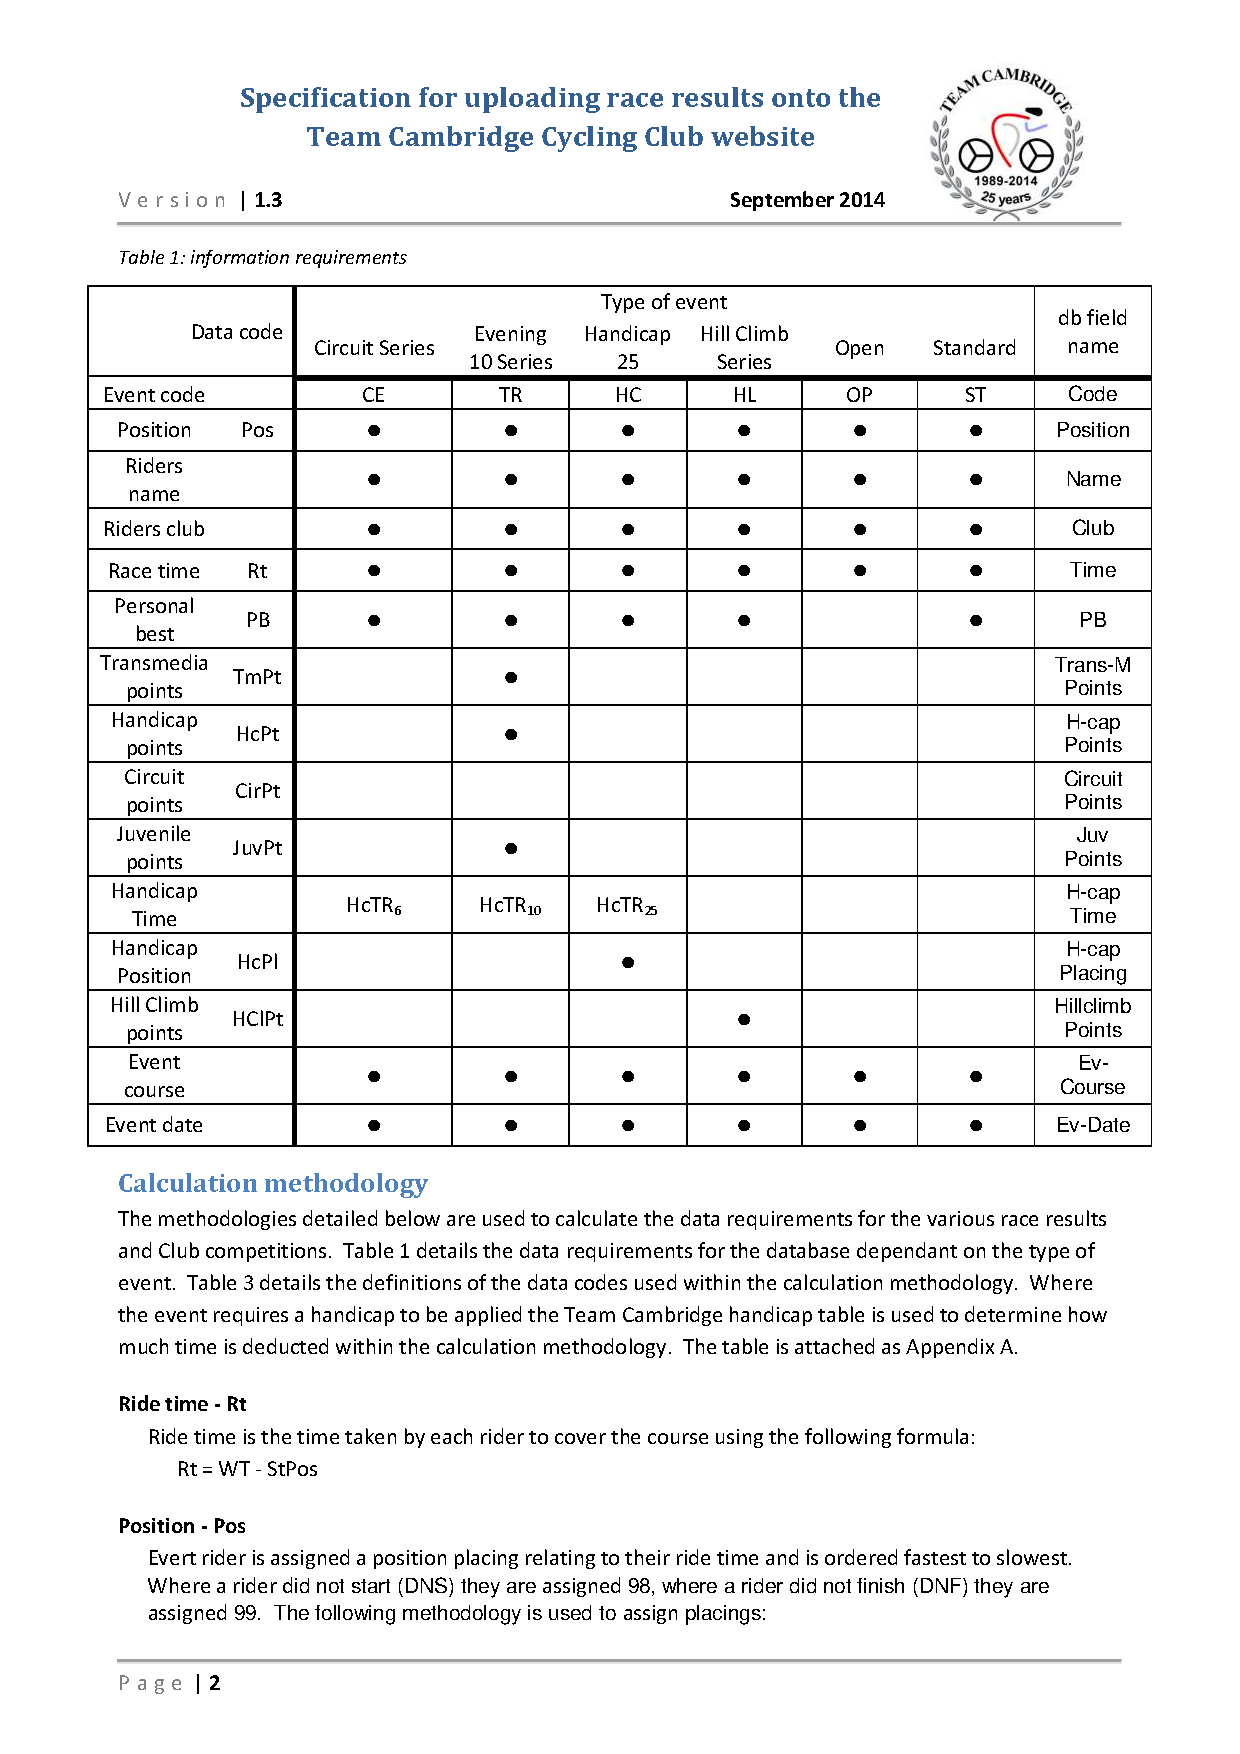
\includegraphics[width=\textwidth]{./TeamCambridgeSpec/page2.pdf}
\end{figure}

\begin{figure}[H]
    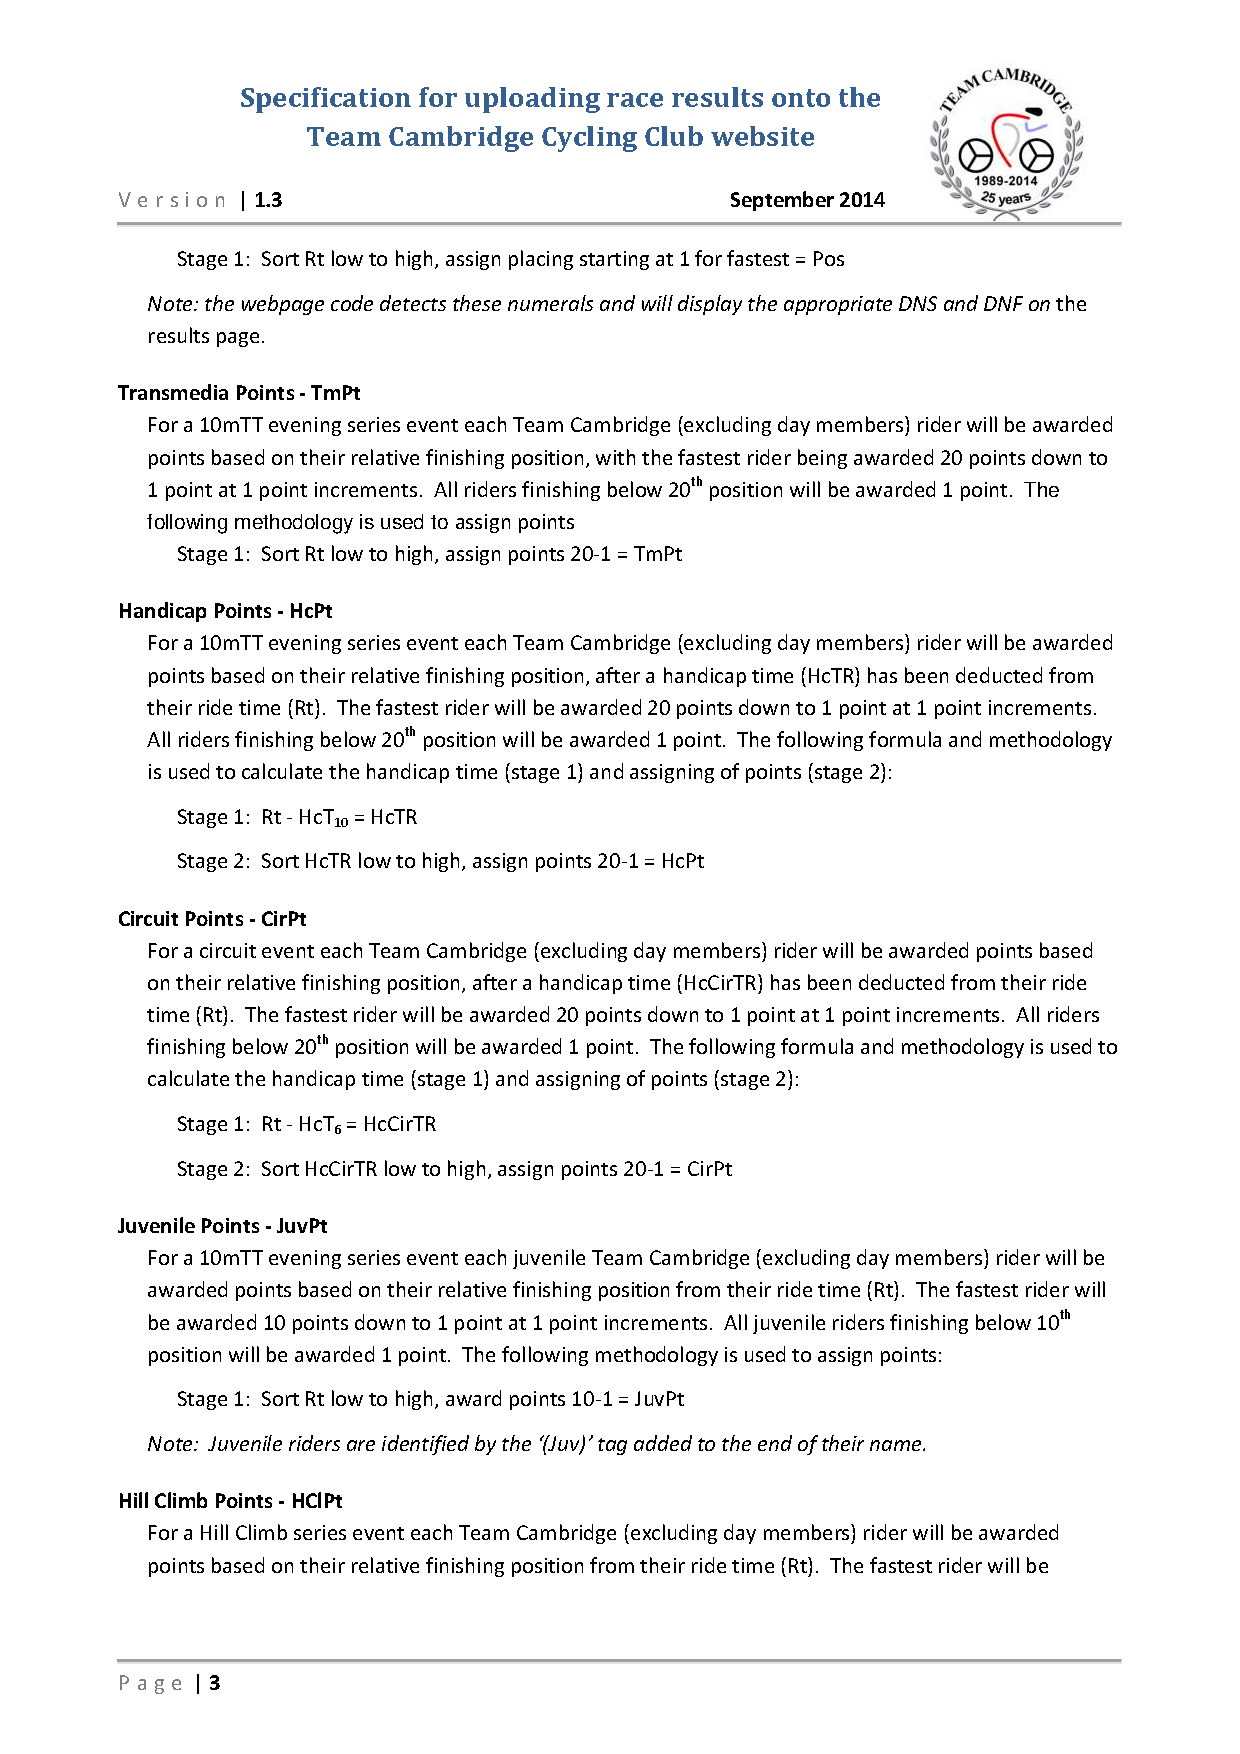
\includegraphics[width=\textwidth]{./TeamCambridgeSpec/page3.pdf}
\end{figure}

\begin{figure}[H]
    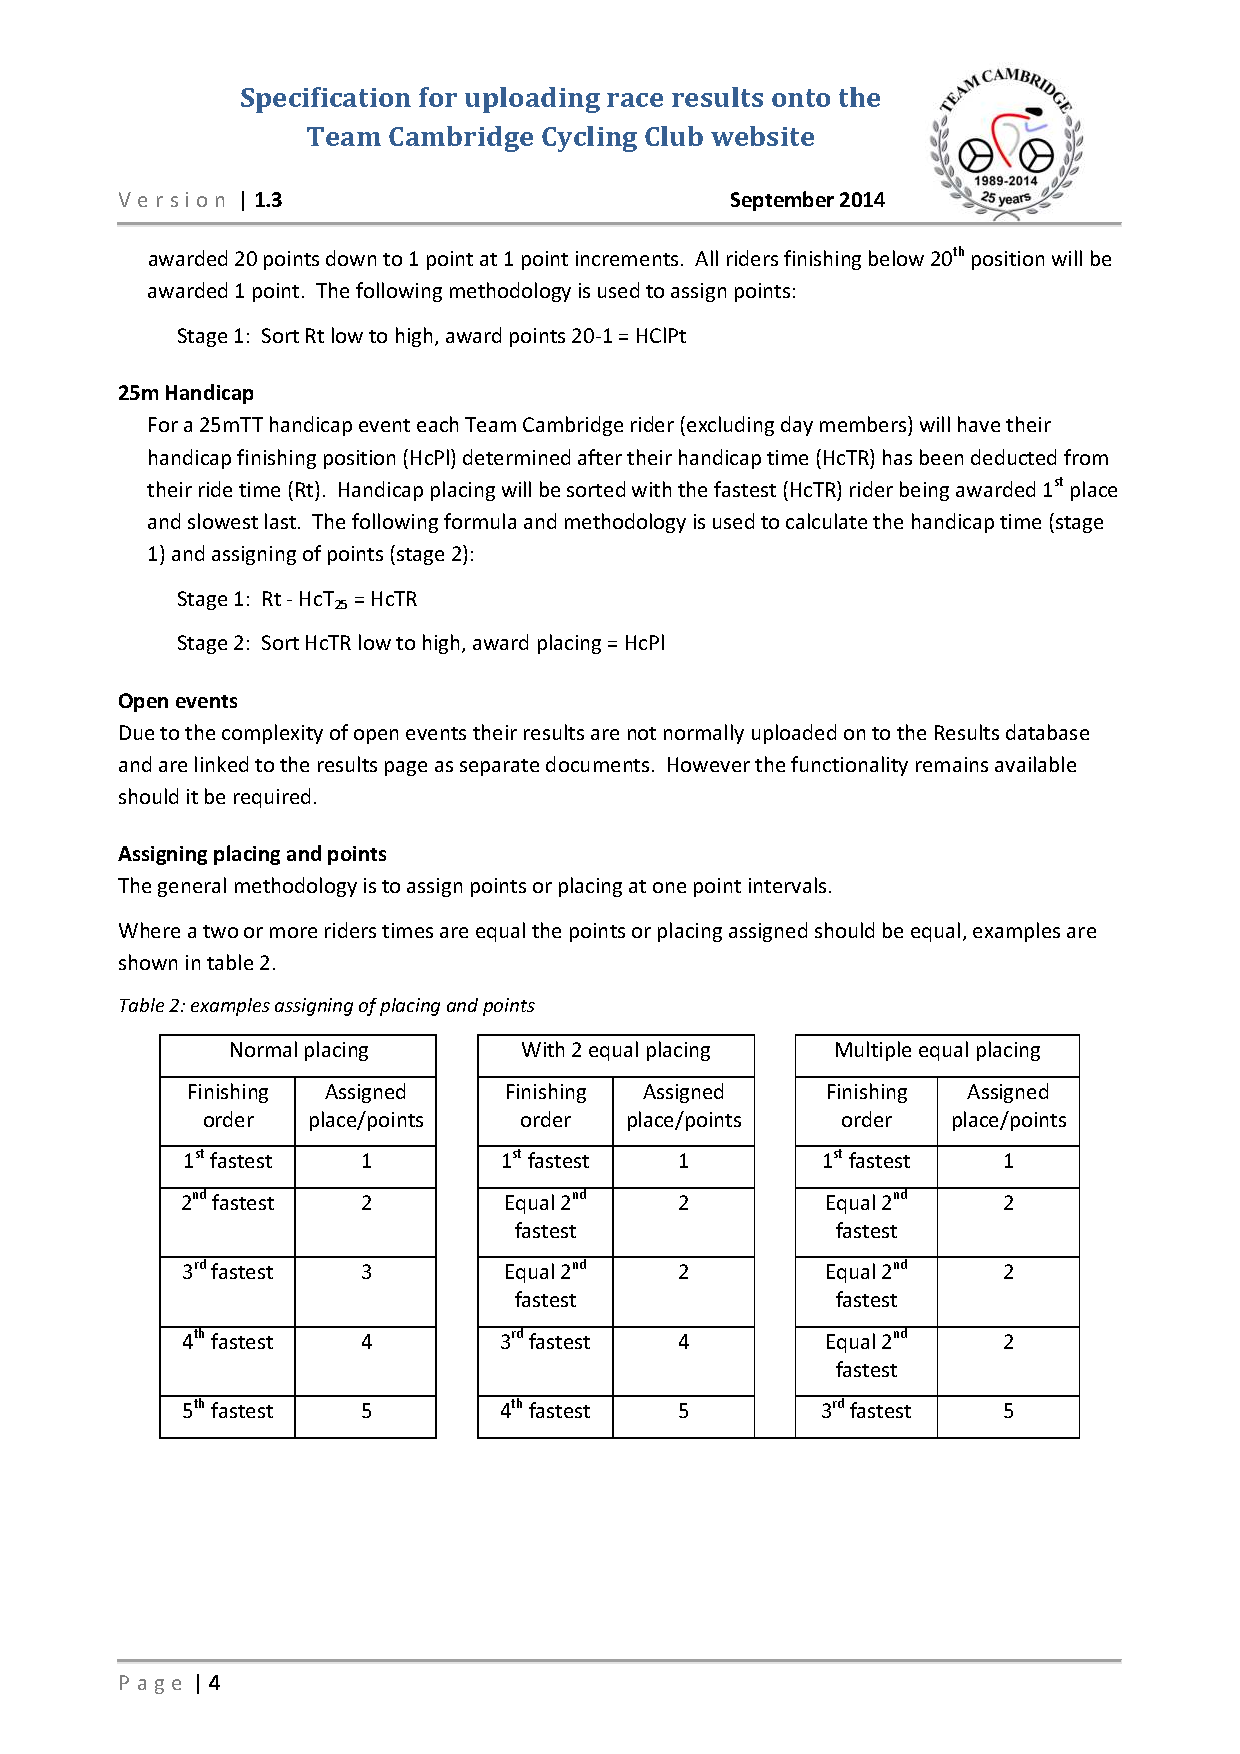
\includegraphics[width=\textwidth]{./TeamCambridgeSpec/page4.pdf}
\end{figure}

\begin{figure}[H]
    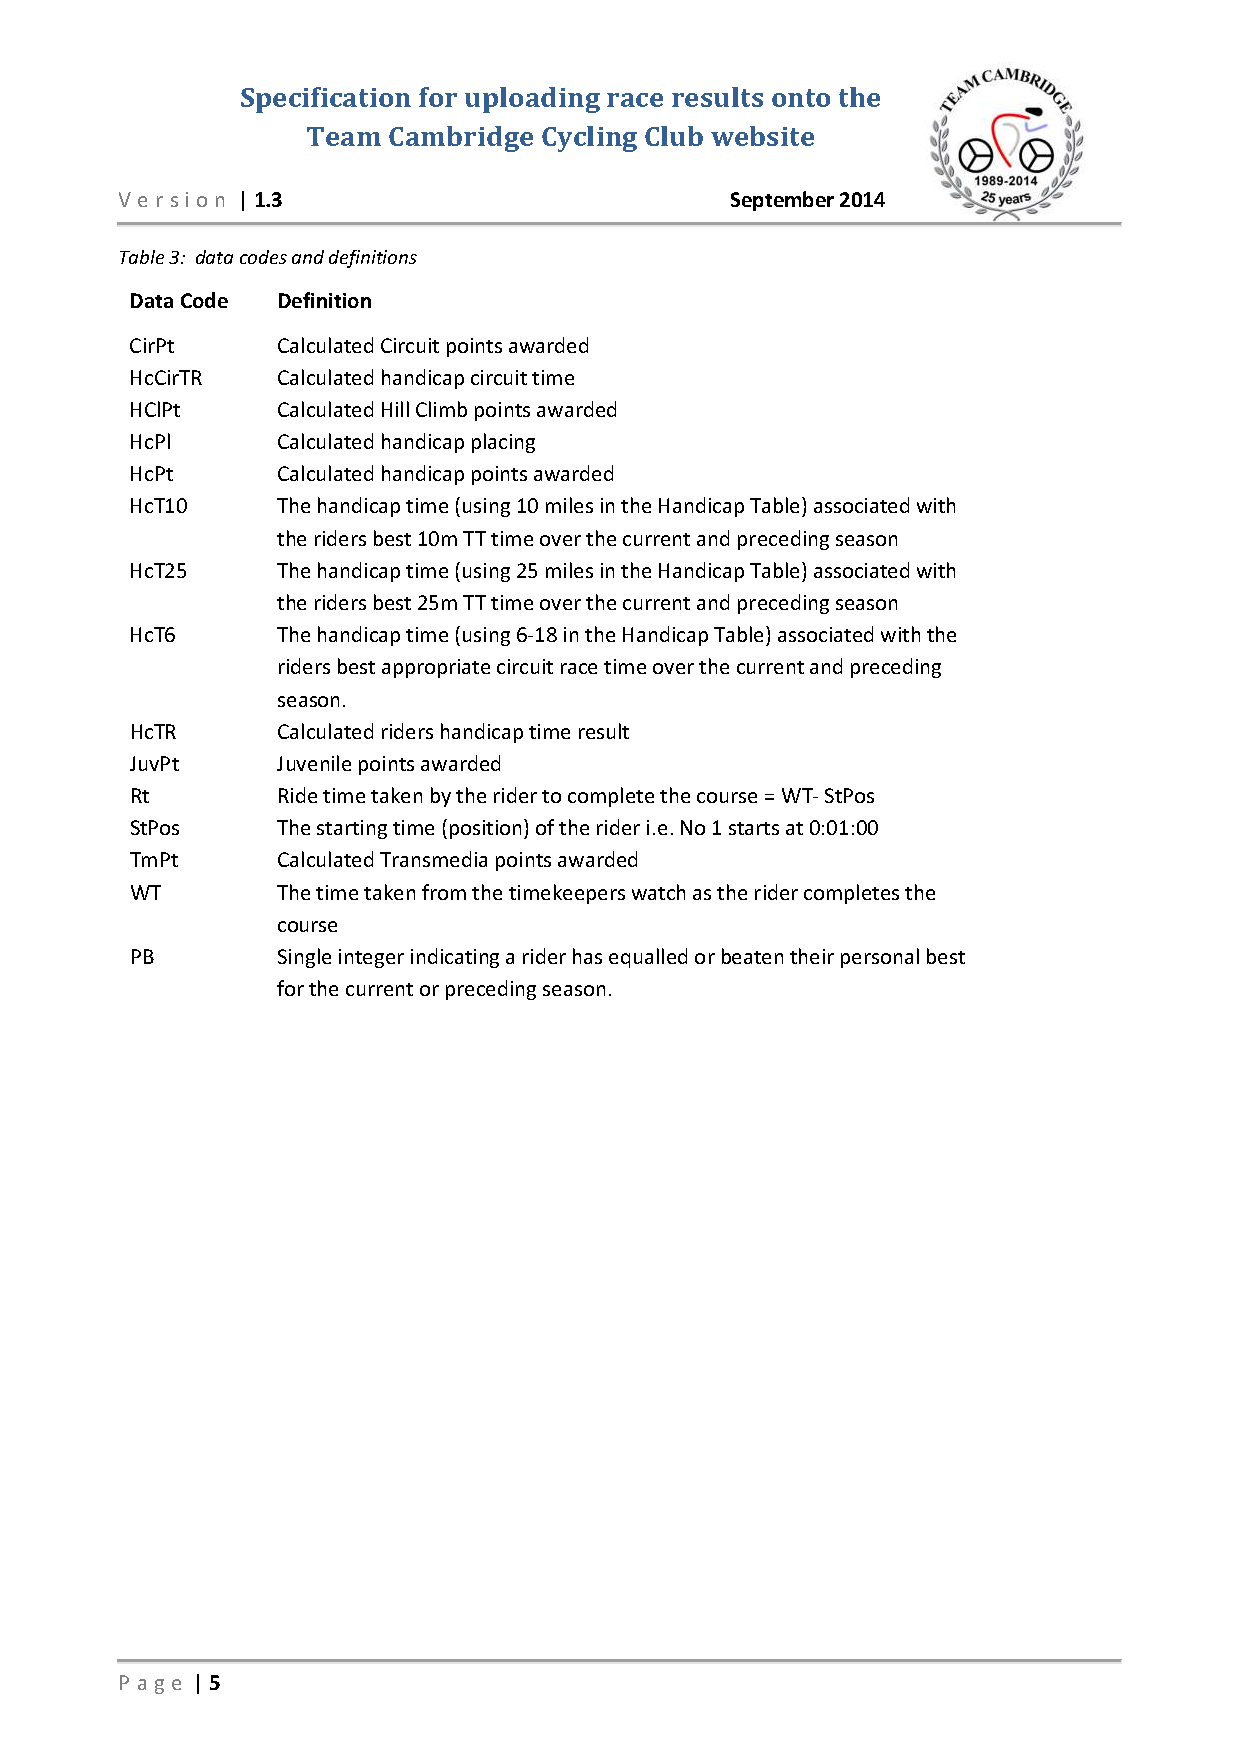
\includegraphics[width=\textwidth]{./TeamCambridgeSpec/page5.pdf}
\end{figure}

\begin{figure}[H]
    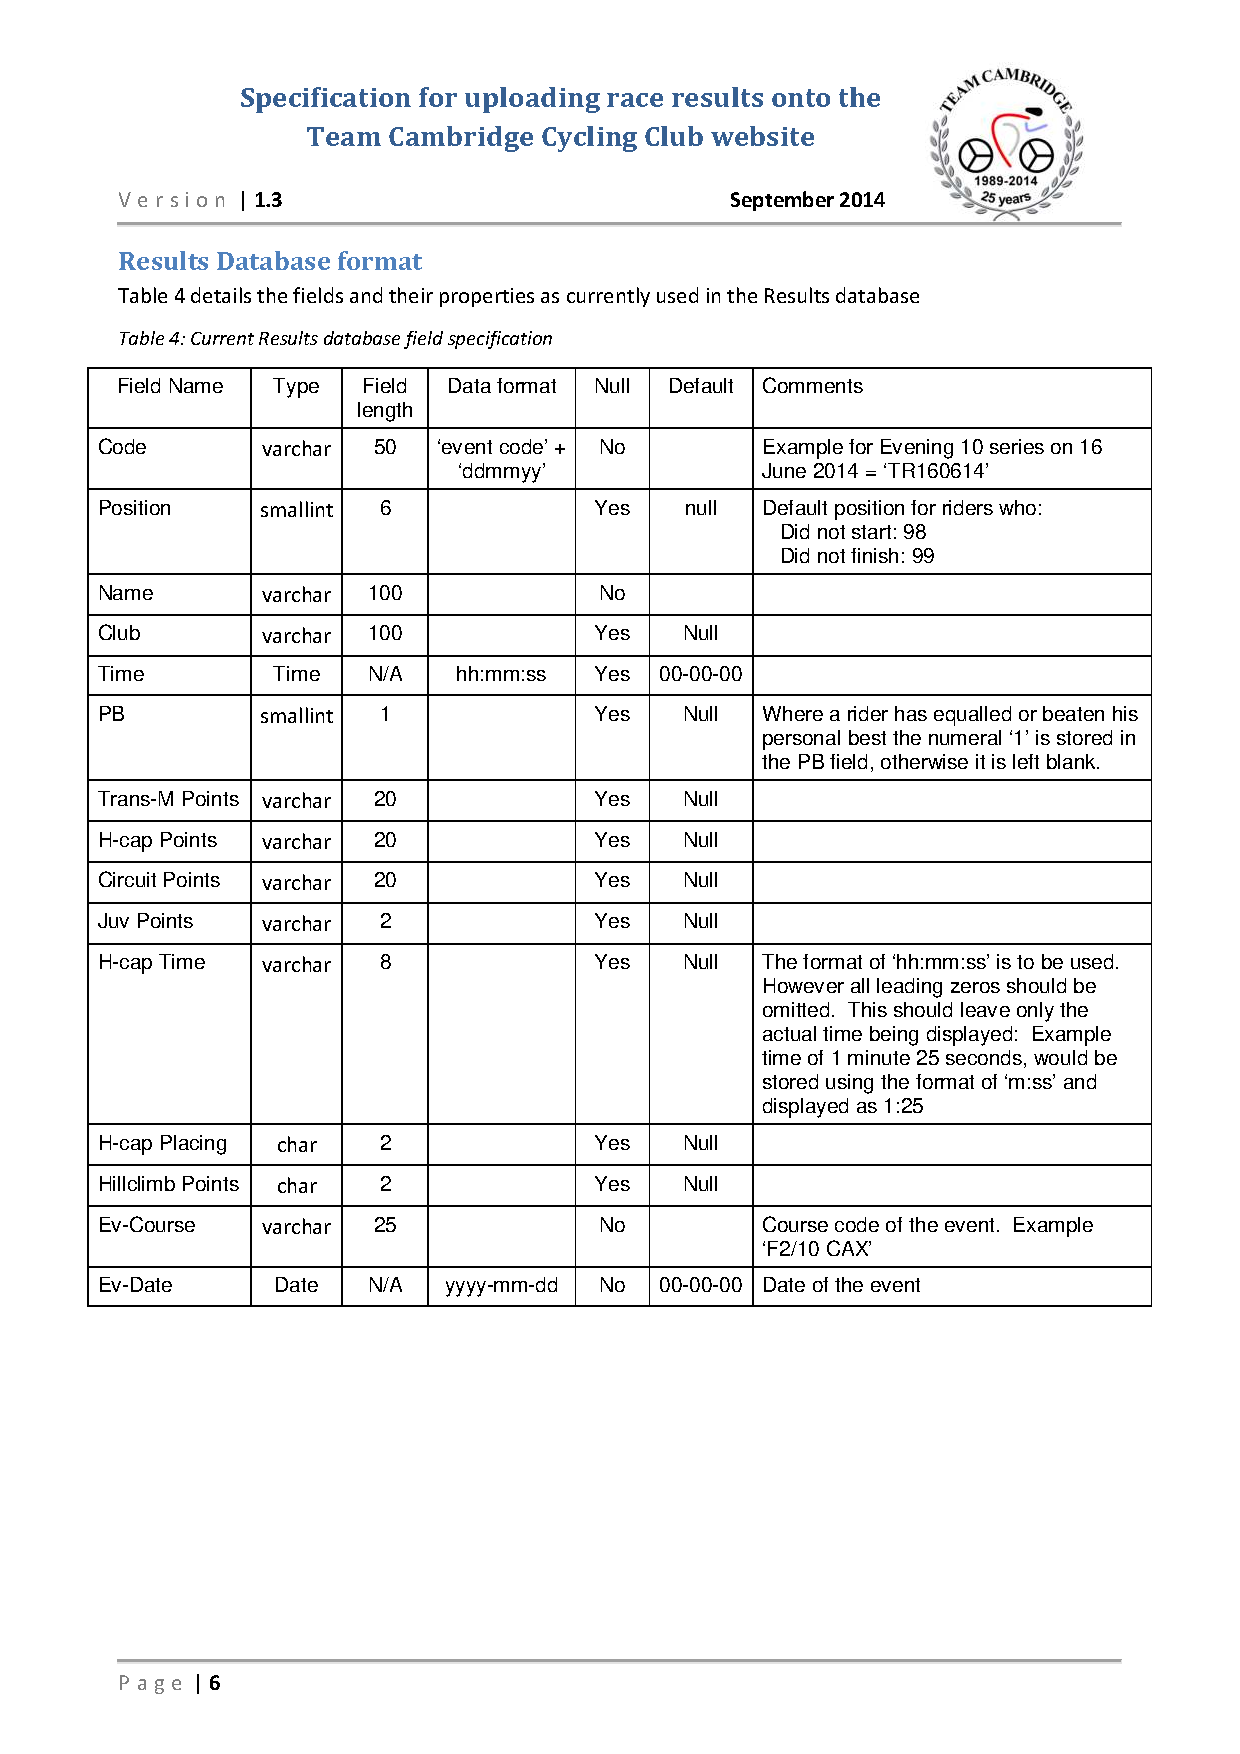
\includegraphics[width=\textwidth]{./TeamCambridgeSpec/page6.pdf}
\end{figure}

\begin{figure}[H]
    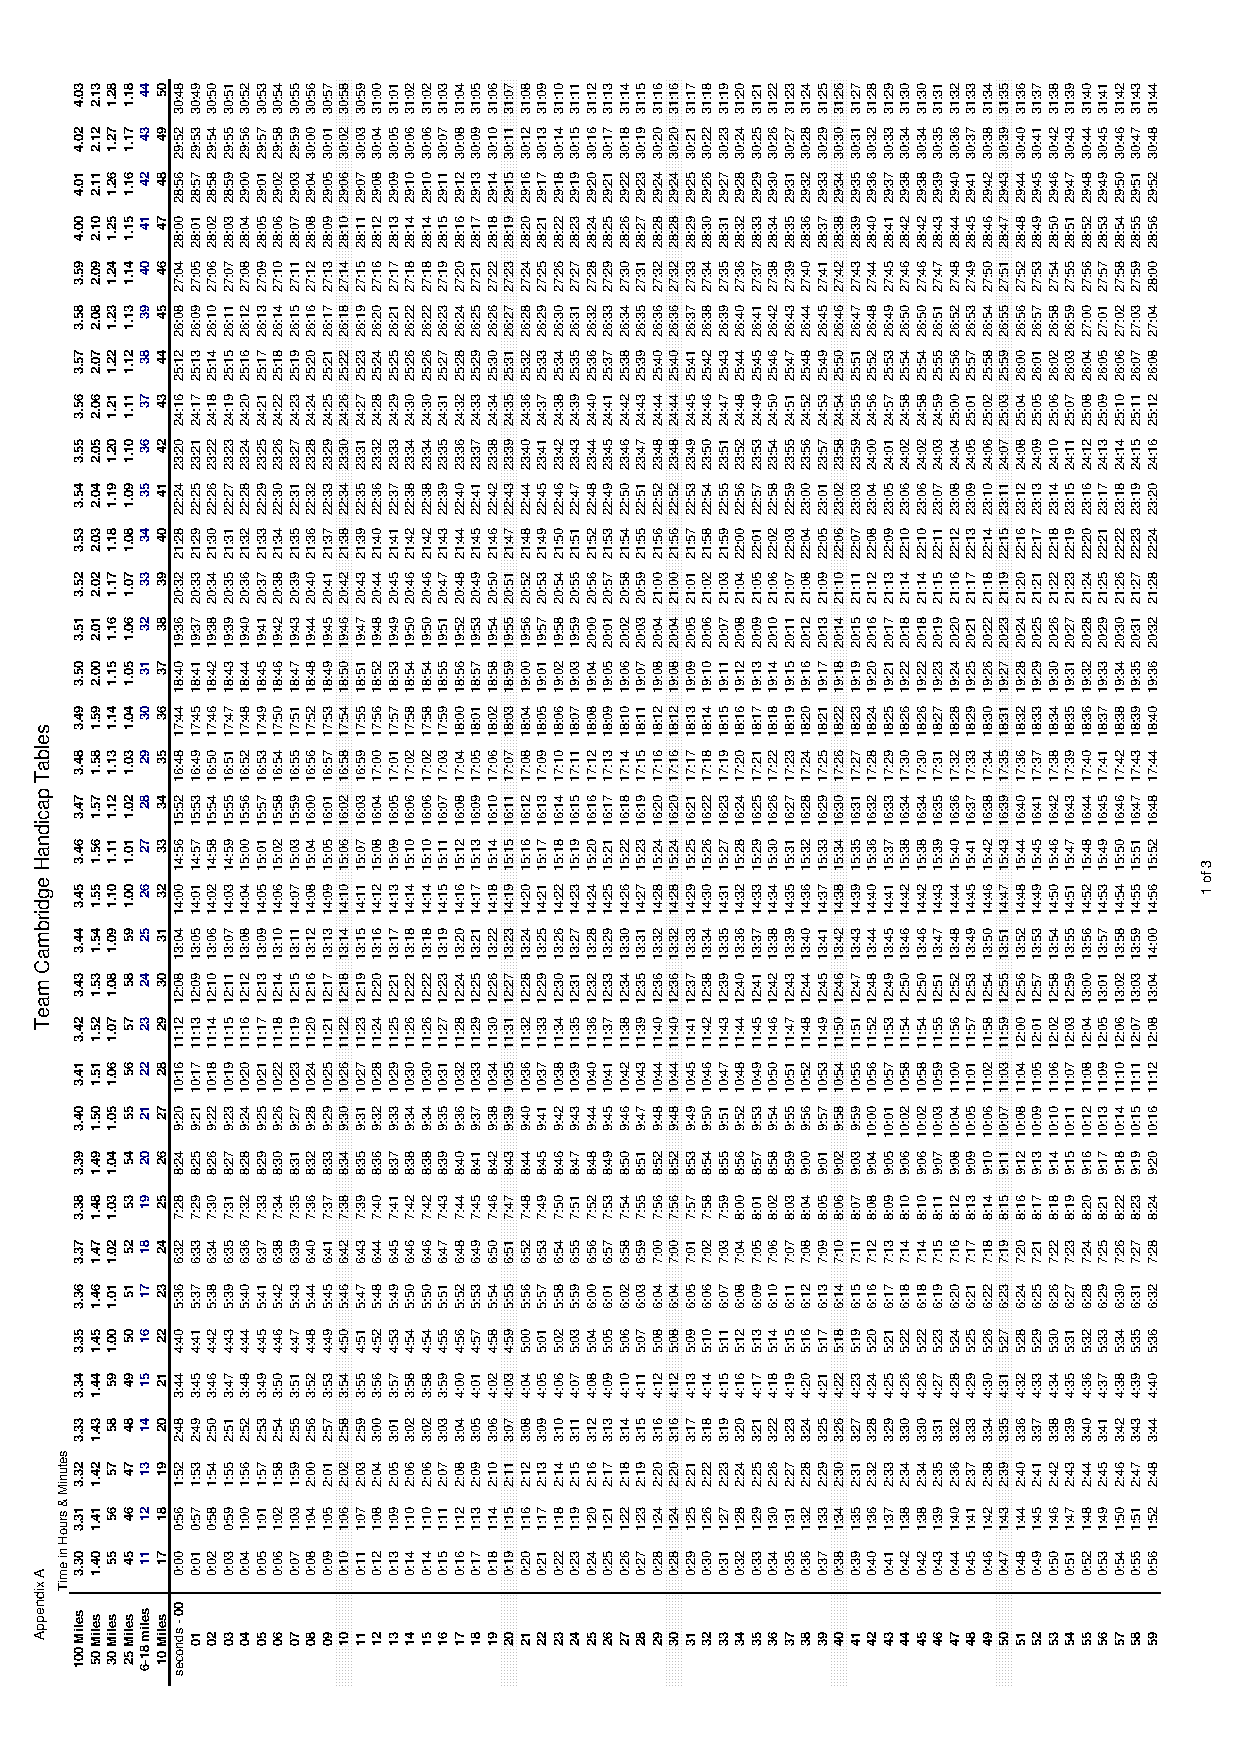
\includegraphics[width=\textwidth]{./TeamCambridgeSpec/page7.pdf}
\end{figure}

\begin{figure}[H]
    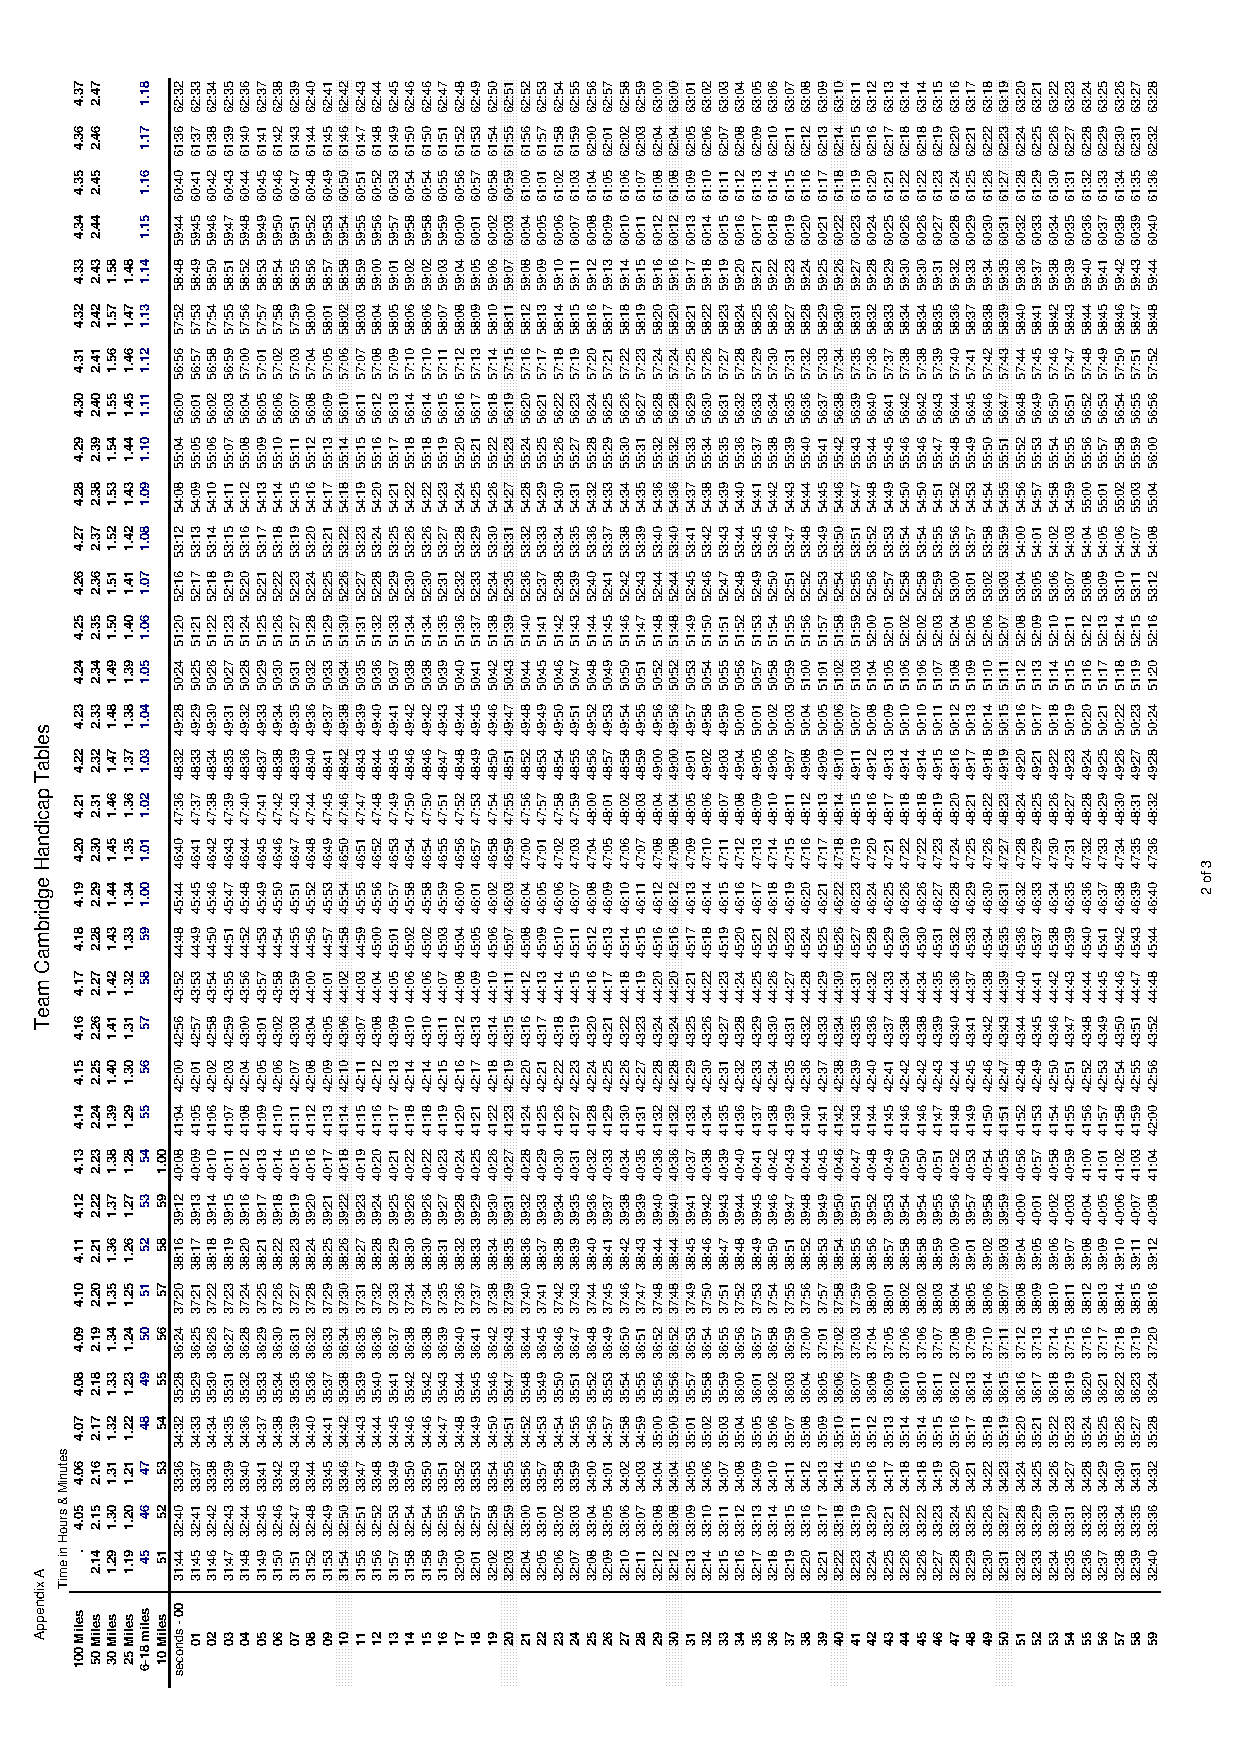
\includegraphics[width=\textwidth]{./TeamCambridgeSpec/page8.pdf}
\end{figure}

\begin{figure}[H]
    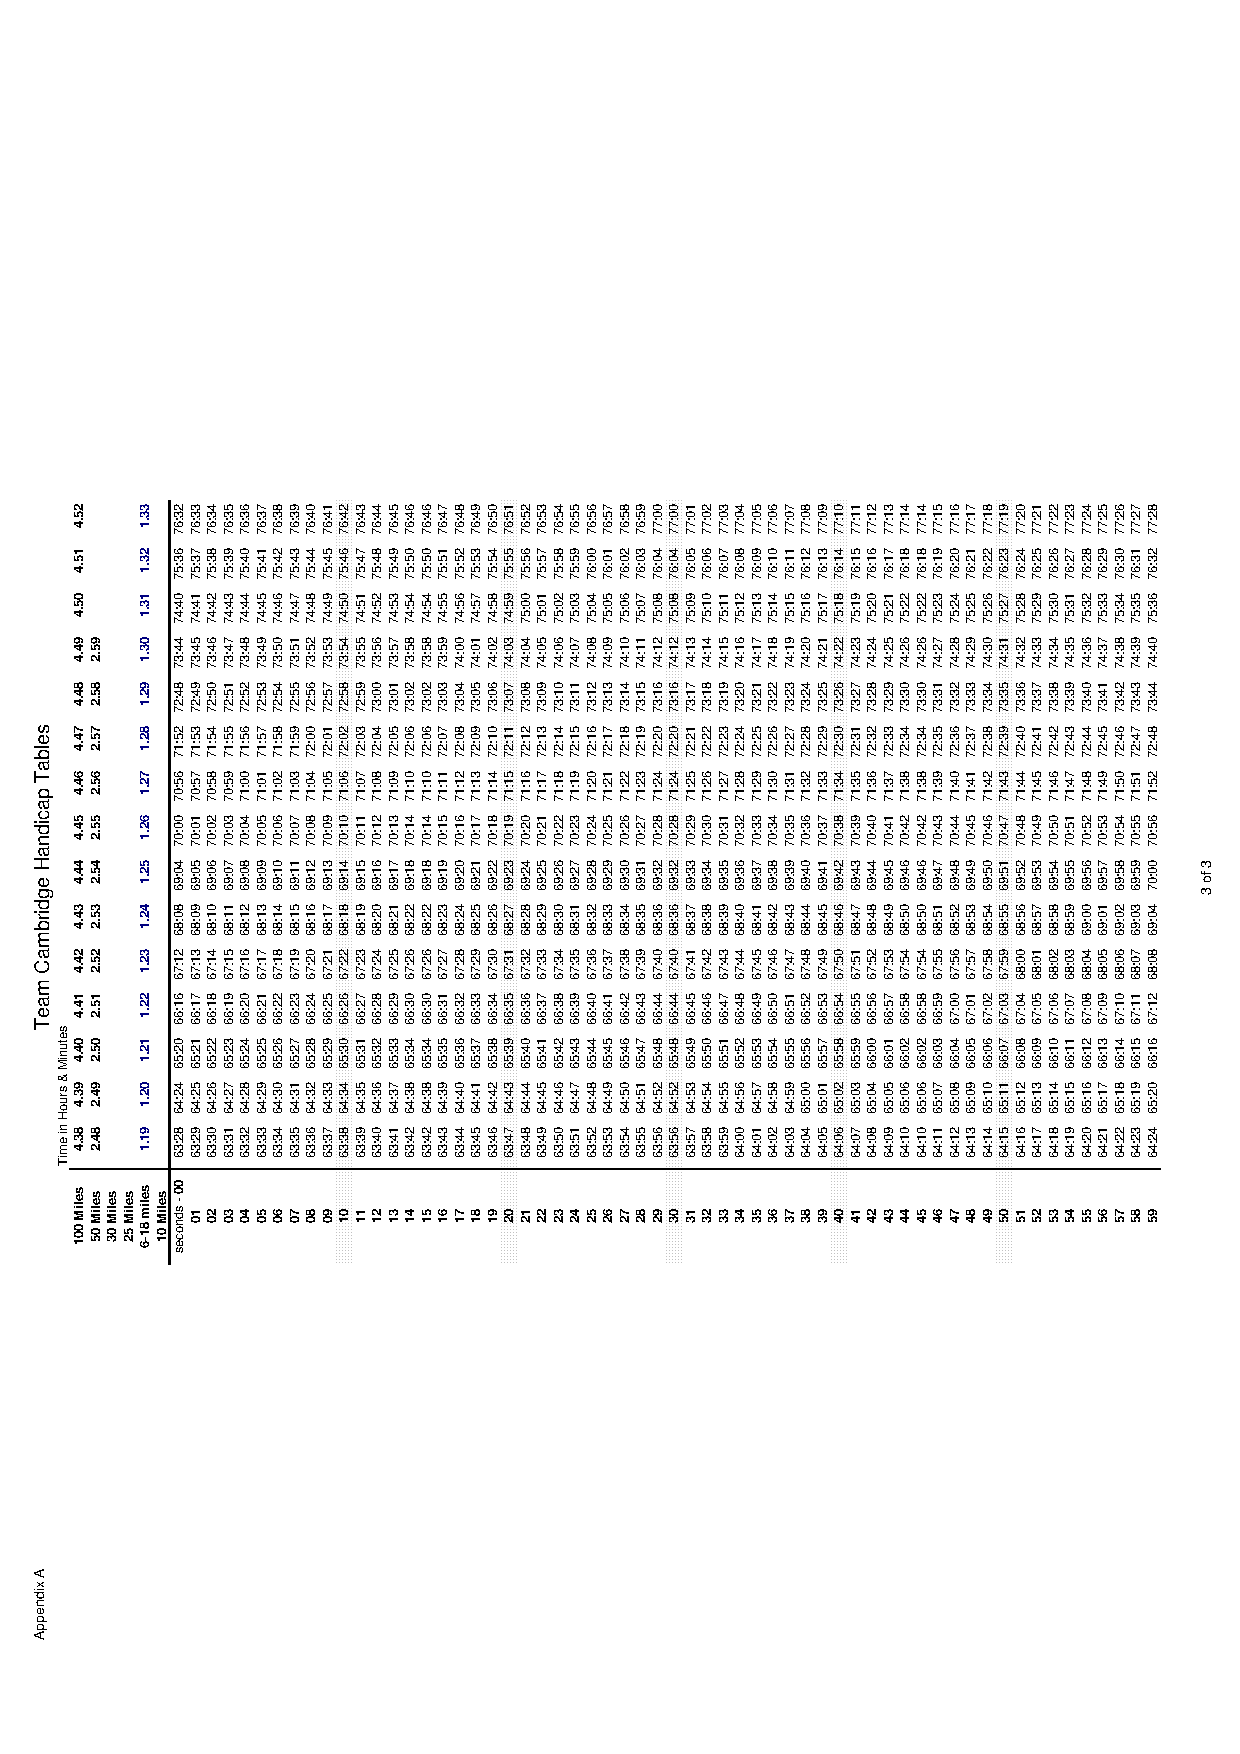
\includegraphics[width=\textwidth]{./TeamCambridgeSpec/page9.pdf}
     \caption{The specification supplied by Paul Millard} \label{fig:Specification}
\end{figure}



The interview questions and notes taken from answers.

\begin{figure}[H]

    \includegraphics[width=\textwidth]{./Questions.pdf}

    \includegraphics[width=\textwidth]{./TeamCambridgeSpec/Questions.pdf}

    \caption{The Questions that I asked Paul Millard in our interview} \label{fig:Questions}
\end{figure}





\begin{figure}[H]
    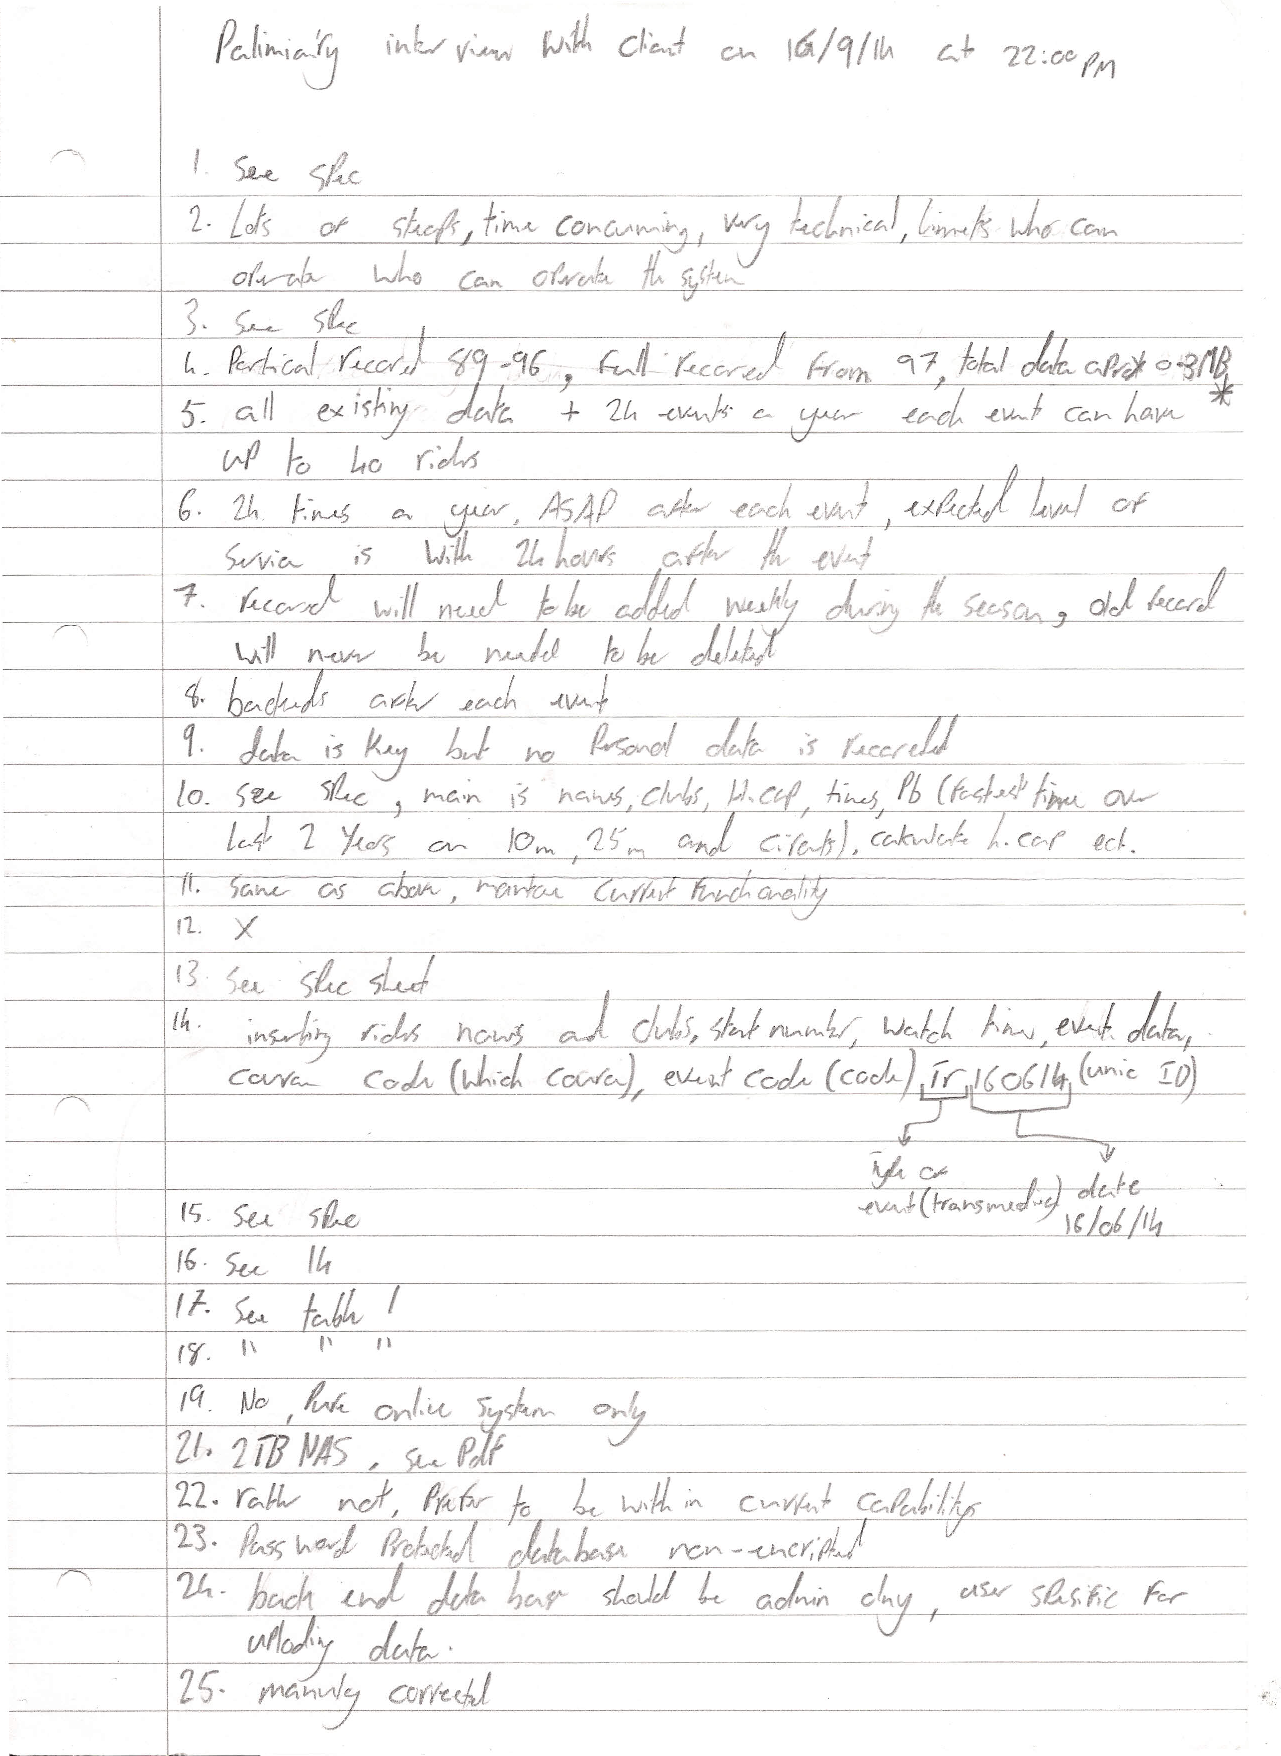
\includegraphics[width=\textwidth]{./interview/InterviewNotesPage1.pdf}
\end{figure}

\begin{figure}[H]
    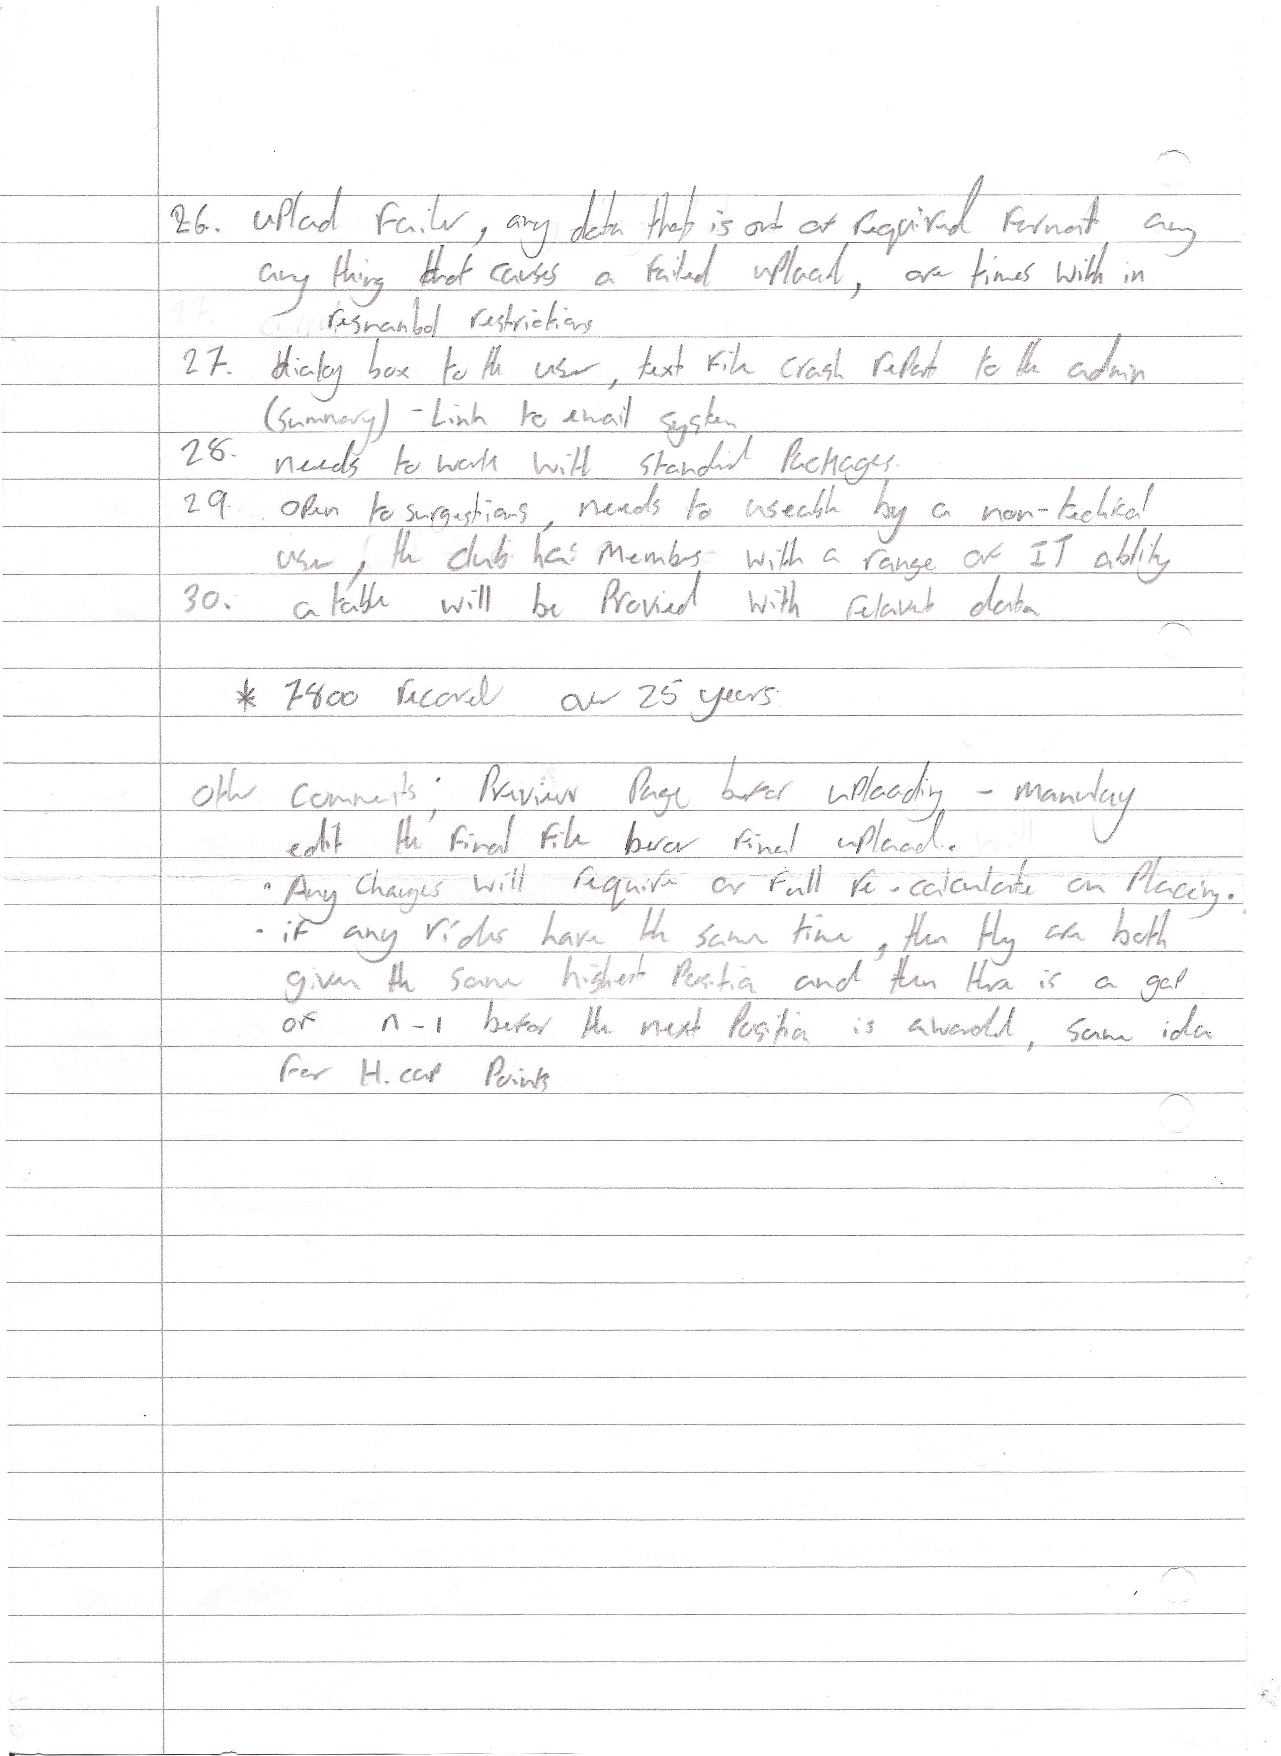
\includegraphics[width=\textwidth]{./interview/InterviewNotesPage2.pdf}
    \caption{The notes taken from the interview with Paul Millard} \label{fig:Interview notes}
\end{figure}


\section{Investigation}

\subsection{The current system}

\subsubsection{Data sources and destinations}

There are currently two sources of data used in the system, the race results from the Time Keepers and the database, also a look up table is used to find the handicap times. For any handicap events both sources of data is needed for all other event only the results are required. The only data destination is the database.

There are currently four data sources; the rider, Timekeeper, Racing Secretary and the database. The rider fills in their personal information on the signing-on sheet and the Timekeepers complete the watch time and ride time sections of the form. A lookup table is used when handicap times need to be calculated for handicap competitions together with the race results and the database. For all other competitions only the race results are required. Any data that needs to be stored is saved in the existing database.

The data from the results are on a paper form that the time keepers use during the events an example of one below shows that there are 8 fields, name and Address, No. , Watch Time, Emergency Tel., Club, Age, Signature. Of these fields only Name, No., Watch Time, Club and Age (if the rider is under the age of 18) are recorded in the database. As for the database the only information that is needed from it is the riders personal best time

The signing-on sheet is a paper form for the race results which after the event is given to the Racing Secretary. An example of this form can be found  in the "Input Forms, Output Forms, Report Formats section". From the form only Name, Club, Watch Time and Age (if under 18) are recorded in the existing database. The current database is a web hosted SQL database accessed though cPanel that was built by Paul Millard. 

This information is used to calculate the points that the riders are awarded in the competition(s) that are relevant to the event
=======
All of the data sources in the current database can be found below

All of the data sources in the current database can be found below

\begin{tabular}{|l|l|l|l|}


\hline
DATA & SOURCE & DATA TYPE & DESTINATION \\ \hline
Code & Racing Secretary & String & Algorithm \\ \hline
Position & Racing Secretary & Integer & Algorithm \\ \hline
Name & Rider & String & Racing Secretary \\ \hline
Club & Rider & String & Racing Secretary \\ \hline
Watch Time & Timekeeper & Time & Database \\ \hline
Personal Best & Database & Time & Algorithm \\ \hline
Transmedia Points & Racing Secretary & Integer & Database \\ \hline
Handicap Points & Racing Secretary & Integer & Database \\ \hline
Circuit Points & Racing Secretary & Integer & Database \\ \hline
Juvenile Points & Racing Secretary & Integer & Database \\ \hline
Handicap Time & Racing Secretary & Time & Database \\ \hline
Handicap Placing & Racing Secretary & Integer & Database \\ \hline
Hillclimb Points & Racing Secretary & Integer & Database \\ \hline
Event Course & Timekeeper & Sting & Racing Secretary \\ \hline
Event Date & Timekeeper & Date & Racing Secretary \\ \hline

\end{tabular}

\subsubsection{Algorithms}
The three Algorithms that are used are shown below:

\begin{algorithm}[H]
\label{fig:Ride Time Algorithm}
	\caption{$Ride Time Algorithum$}
\begin{algorithmic}[1]
\RECEIVE{$Watch Time$}
\RECEIVE{$PositionAsTimeValue$}
\SET{$Ride Time$}{$Watch time$}-{$PositionAsTimeValue$}
\end{algorithmic}
\end{algorithm}


* When "Watch Time - Position" is calculated, the "Position" is treated as a time value in minuets, e.g. The rider at "Position" of 13 would have 13 minuets taken off their "Watch Time" to calculate their Ride Time"


\begin{algorithm}[H]
\label{fig:Time Sort Algorithm}
	\caption{$Time Sort Algorithm$}
\begin{algorithmic}[2]
\RECEIVE{$TimeList$}
\SET{$Changes$}{$TRUE$}
\While{$Changes$}{$TRUE$}
	\SET{$Changes$}{$FALSE$}
	\For{$Count$}{$TimeList$}
		\If{$TimeList[Count] > TimeList[Count + 1]$}
			\SET{$Hold$}{$TimeList[count]$}
			\SET{$TimeList[count]$}{$TimeList[Count+1]$}
			\SET{$TimeList[Coutn+1]$}{$Hold$}
		\EndIf
	\EndFor
\EndWhile
\end{algorithmic}
\end{algorithm}

\begin{algorithm}[H]
\label{fig:Handicap Time Algorithm}
	\caption{$Handicap Time Algorithm$}
\begin{algorithmic}[3]
\RECEIVE{$RideTime$}
\RECEIVE{$HandicapModifier$}{$From\ LookupTable$}
\SET{$HndicapTime$}{$Ride Time - HandicapModifier$}
\end{algorithmic}
\end{algorithm}


**The handicap is found from the riders best time for the distance in the last 2 years from a look up table

\begin{algorithm}
\label{fig:Points Awarding Algorithm}
	\caption{$Points Awarding Algorithm$}
\begin{algorithmic}
\SET{$PointToBeAwared$}{$20$}
\RECEIVE{$TimesList$}
\SET{$RiderList$}{$[[Names][points]]$}
\SET{$Counter$}{$0$}
\SET{$Hold$}{$0$}
\SET{$Same$}{$False$}
\For{$Length1$}{$In\ TimeList$}
	\If{$TimeList[Count] = TimeList[Count + 1]$}
		\SET{$Hold$}{$2$}
		\SET{$Same$}{$True$}
		\SET{$Count$}{$Count + 1$}
		\While{$Same$}{$True$}
			\If{$TimeList[Count] = TimeList[Count+1]$}
				\SET{$Same$}{$True$}
				\SET{$Hold$}{$Hold + 1$}
			\Else
				\SET{$Same$}{$False$}
			\EndIf
		\EndWhile
	\EndIf
	\If{$Hold NOT 0$}
		\SET{$Mod$}{$0$}
		\For{$Length2$}{$In\ Hold$}
			\SET{$RiderList[[None][Count - Hold + Mod]]$}{$PointToBeAwared$}
			\SET{$Mod$}{$Mod + 1$}
		\EndFor
		\SET{$PointToBeAwared$}{$PointToBeAwared - 1$}
		\SET{$Count$}{$Count + 1$}\textbf{}
	\Else
		\SET{$RiderList[[None][Count]]$}{$PointToBeAwared$}
		\SET{$PointToBeAwared$}{$PointToBeAwared - 1$}
		\SET{$Count$}{$Count + 1$}
	\EndIf
\EndFor
\end{algorithmic}
\end{algorithm}

\subsubsection{Data flow diagram}\i

This is the data flow diagram for add the results of a handicap event.



\begin{figure}[H]
    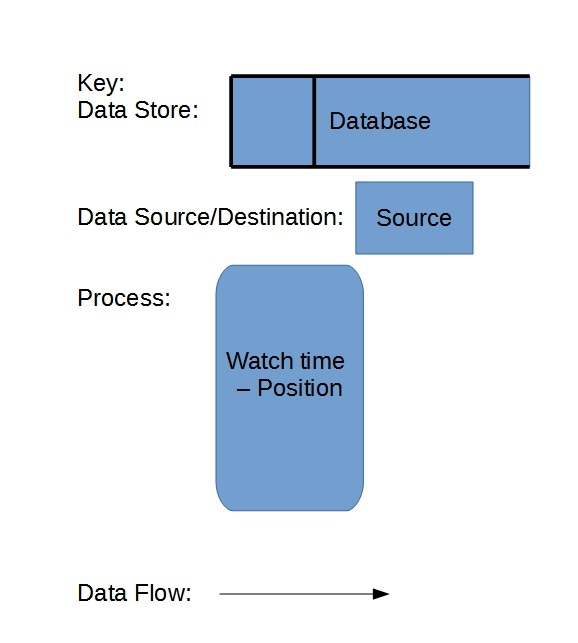
\includegraphics[width=\textwidth]{./DFD/Done/JPG/DFDKey.jpg}
    \caption{DFD Key} \label{fig:DFD key}
\end{figure}


This is the data flow diagram for adding a non-handicap even.

\begin{figure}[H]
    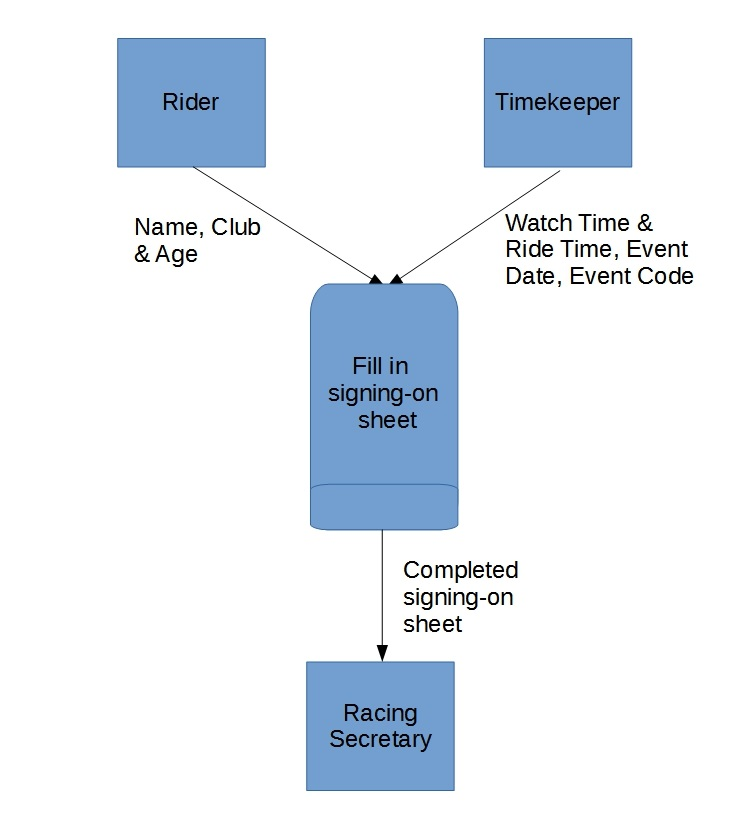
\includegraphics[width=\textwidth]{./DFD/Done/JPG/DataCollection.jpg}
    \caption{Data collection DFD} \label{fig:Data collection DFD}
\end{figure}

\begin{figure}[H]
    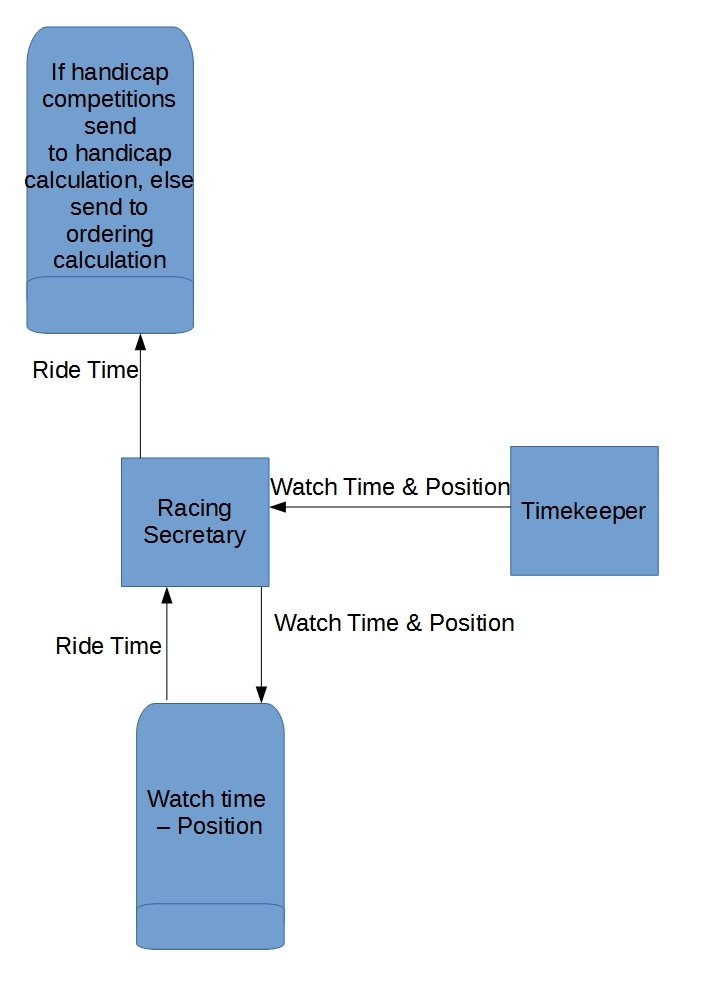
\includegraphics[width=\textwidth]{./DFD/Done/JPG/RideTimeDFD.jpg}
    \caption{Ride time DFD} \label{fig:Ride time calculation DFD}
\end{figure}

\begin{figure}[H]
    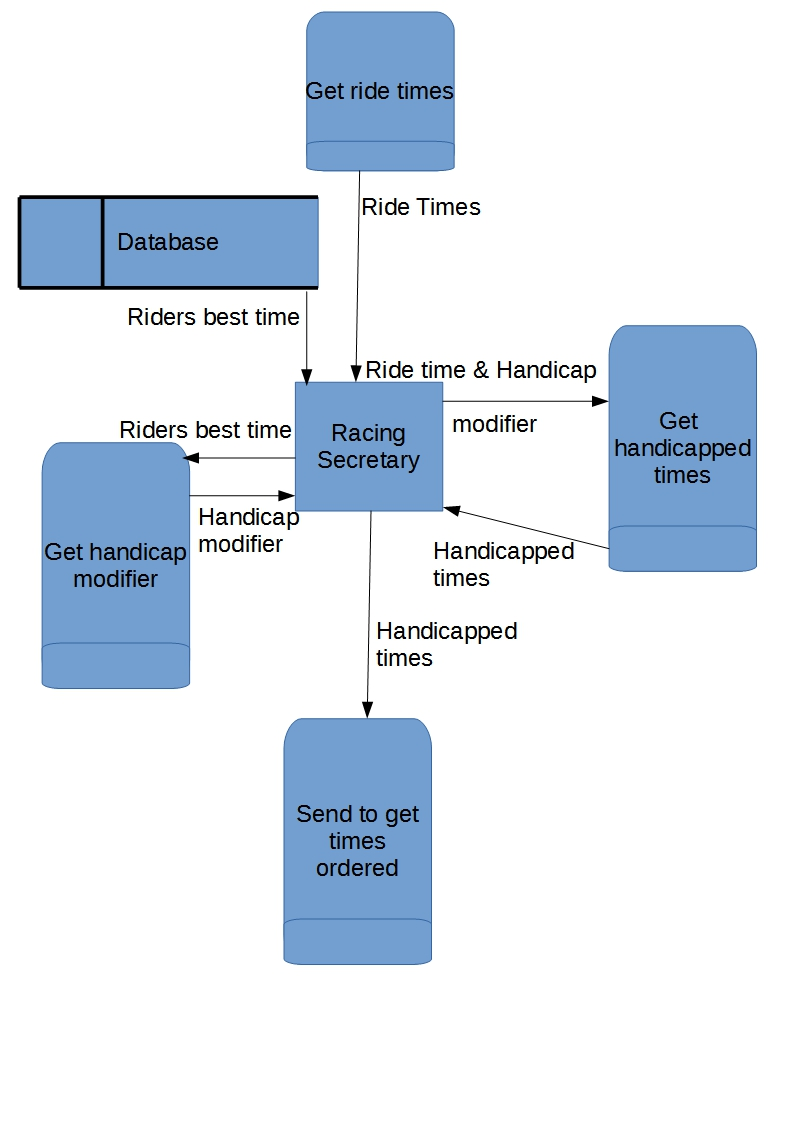
\includegraphics[width=\textwidth]{./DFD/Done/JPG/HandicapDFD.jpg}
    \caption{Handicap calculation DFD} \label{fig:Handicap Calculation DFD}
\end{figure}

\begin{figure}[H]
    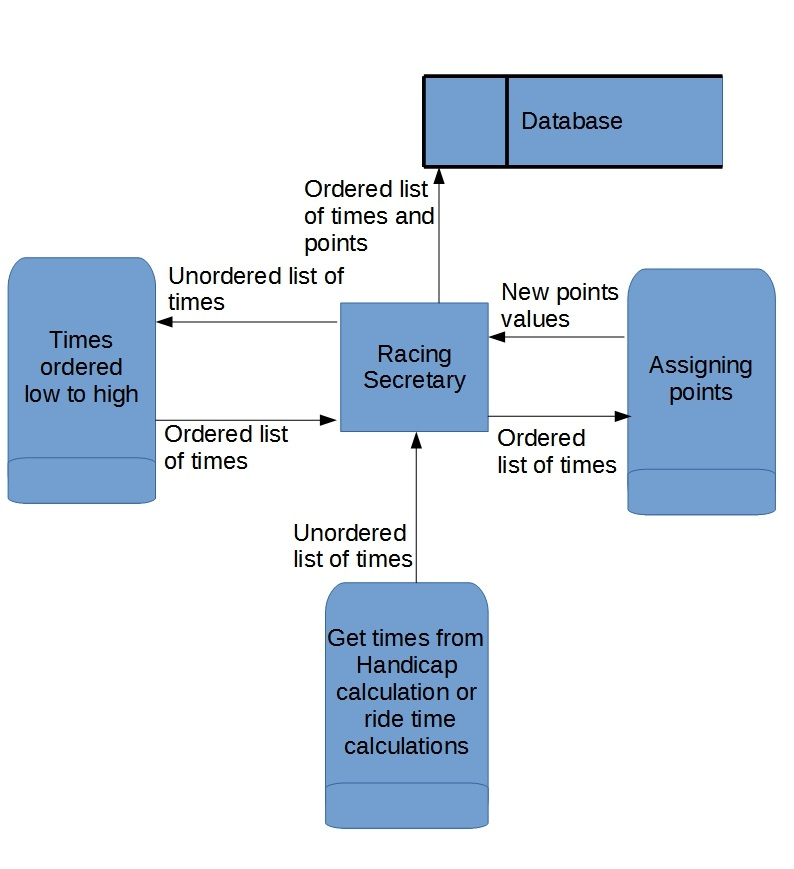
\includegraphics[width=\textwidth]{./DFD/Done/JPG/OrderingTimes.jpg}
    \caption{Ordering Times DFD} \label{fig:Orgering times DFD}
\end{figure}


\subsubsection{Input Forms, Output Forms, Report Formats}
The current system only has one form, the sign on sheet. It's used by the Time Keepers on the day of the event, the fields on the form are "Name", "No.", "Watch Time", "Emergency Tel.", "Club", "Age", "Signature", "Course" and "Date".

\begin{figure}[H]
    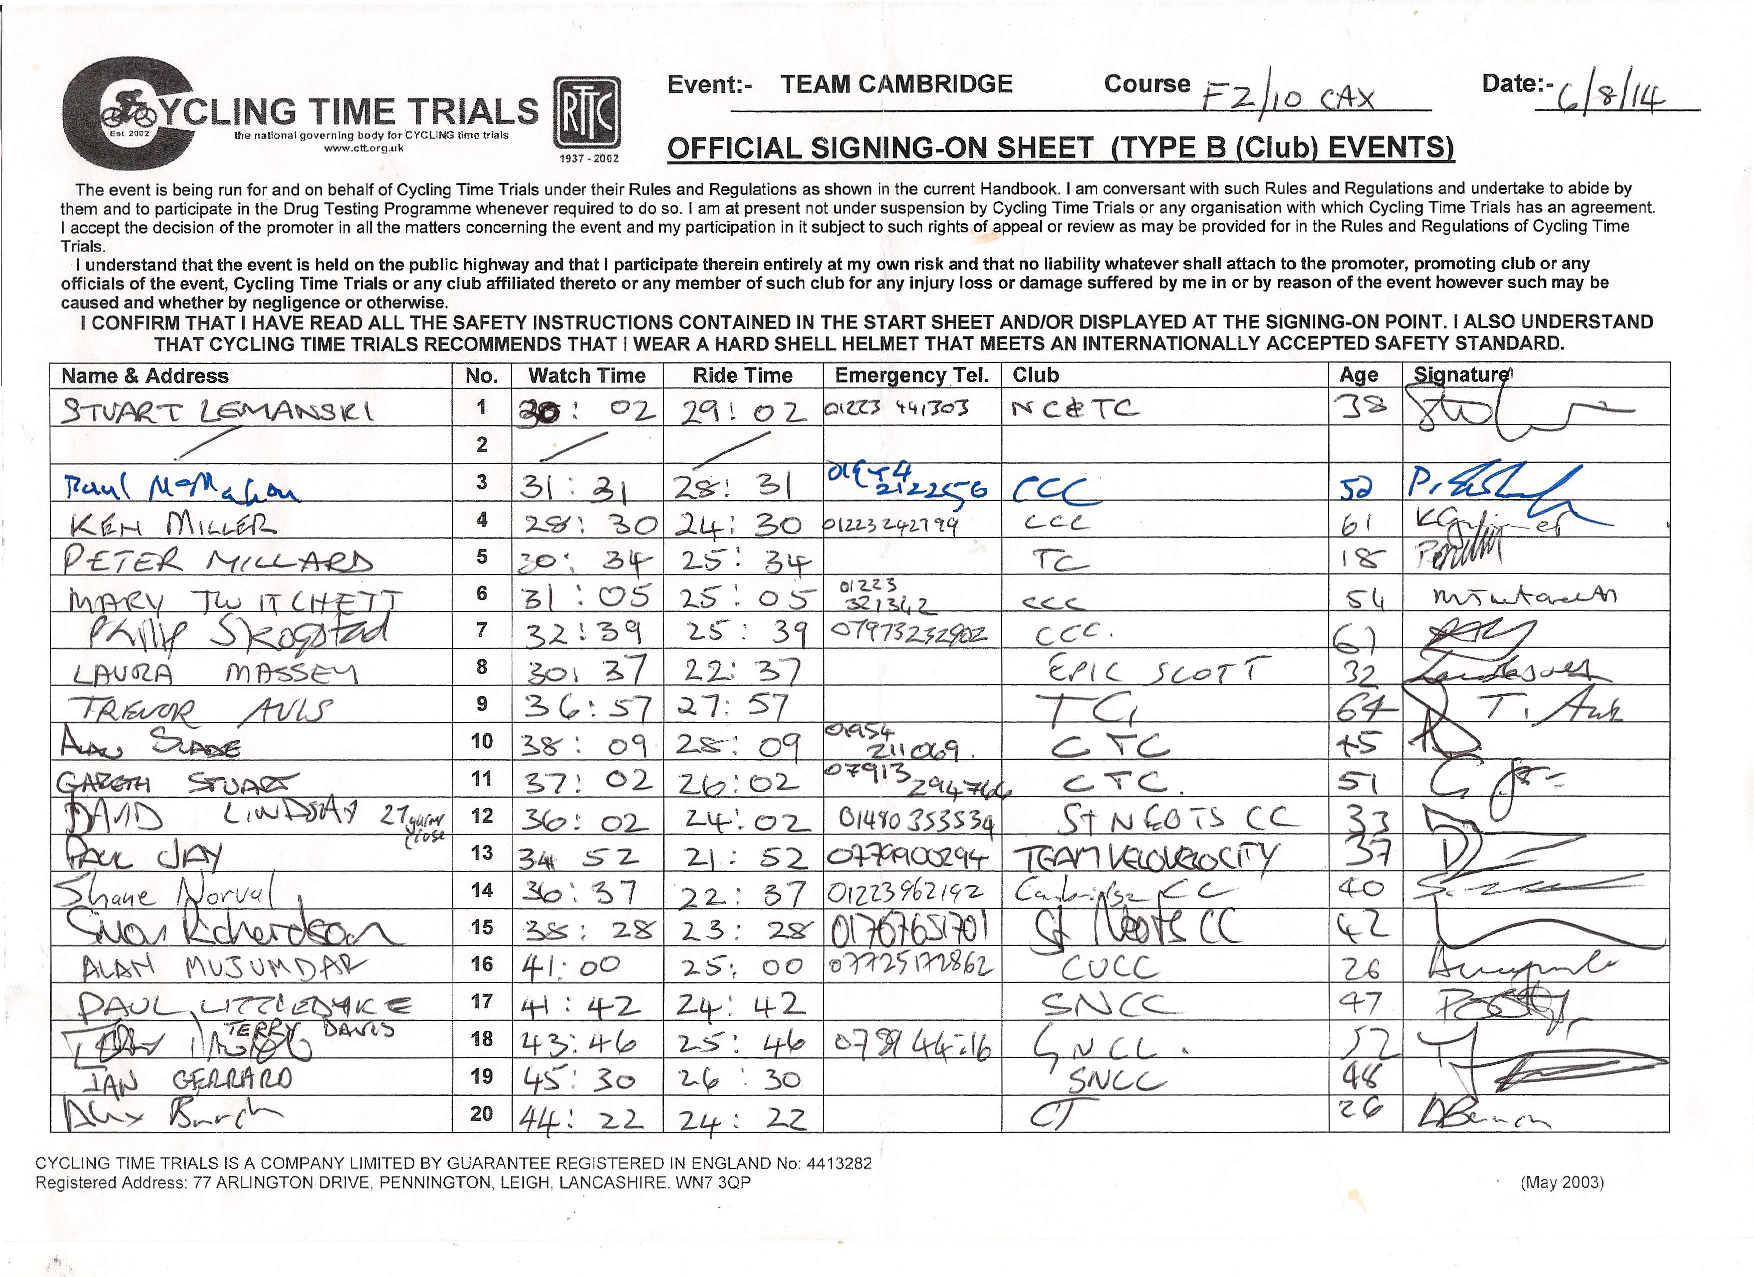
\includegraphics[width=\textwidth]{./SignOnTimeKeepersSheet.pdf}
    \caption{Example fo the signing-on sheet} \label{fig:Example fo the signing-on sheet}
\end{figure}

\subsubsection{Data sources and destinations}

The data sources and destination of the proposed system are very slimier to the current system as the project aims to automate the current system rather than change the current one.

\begin{figure}[H]
	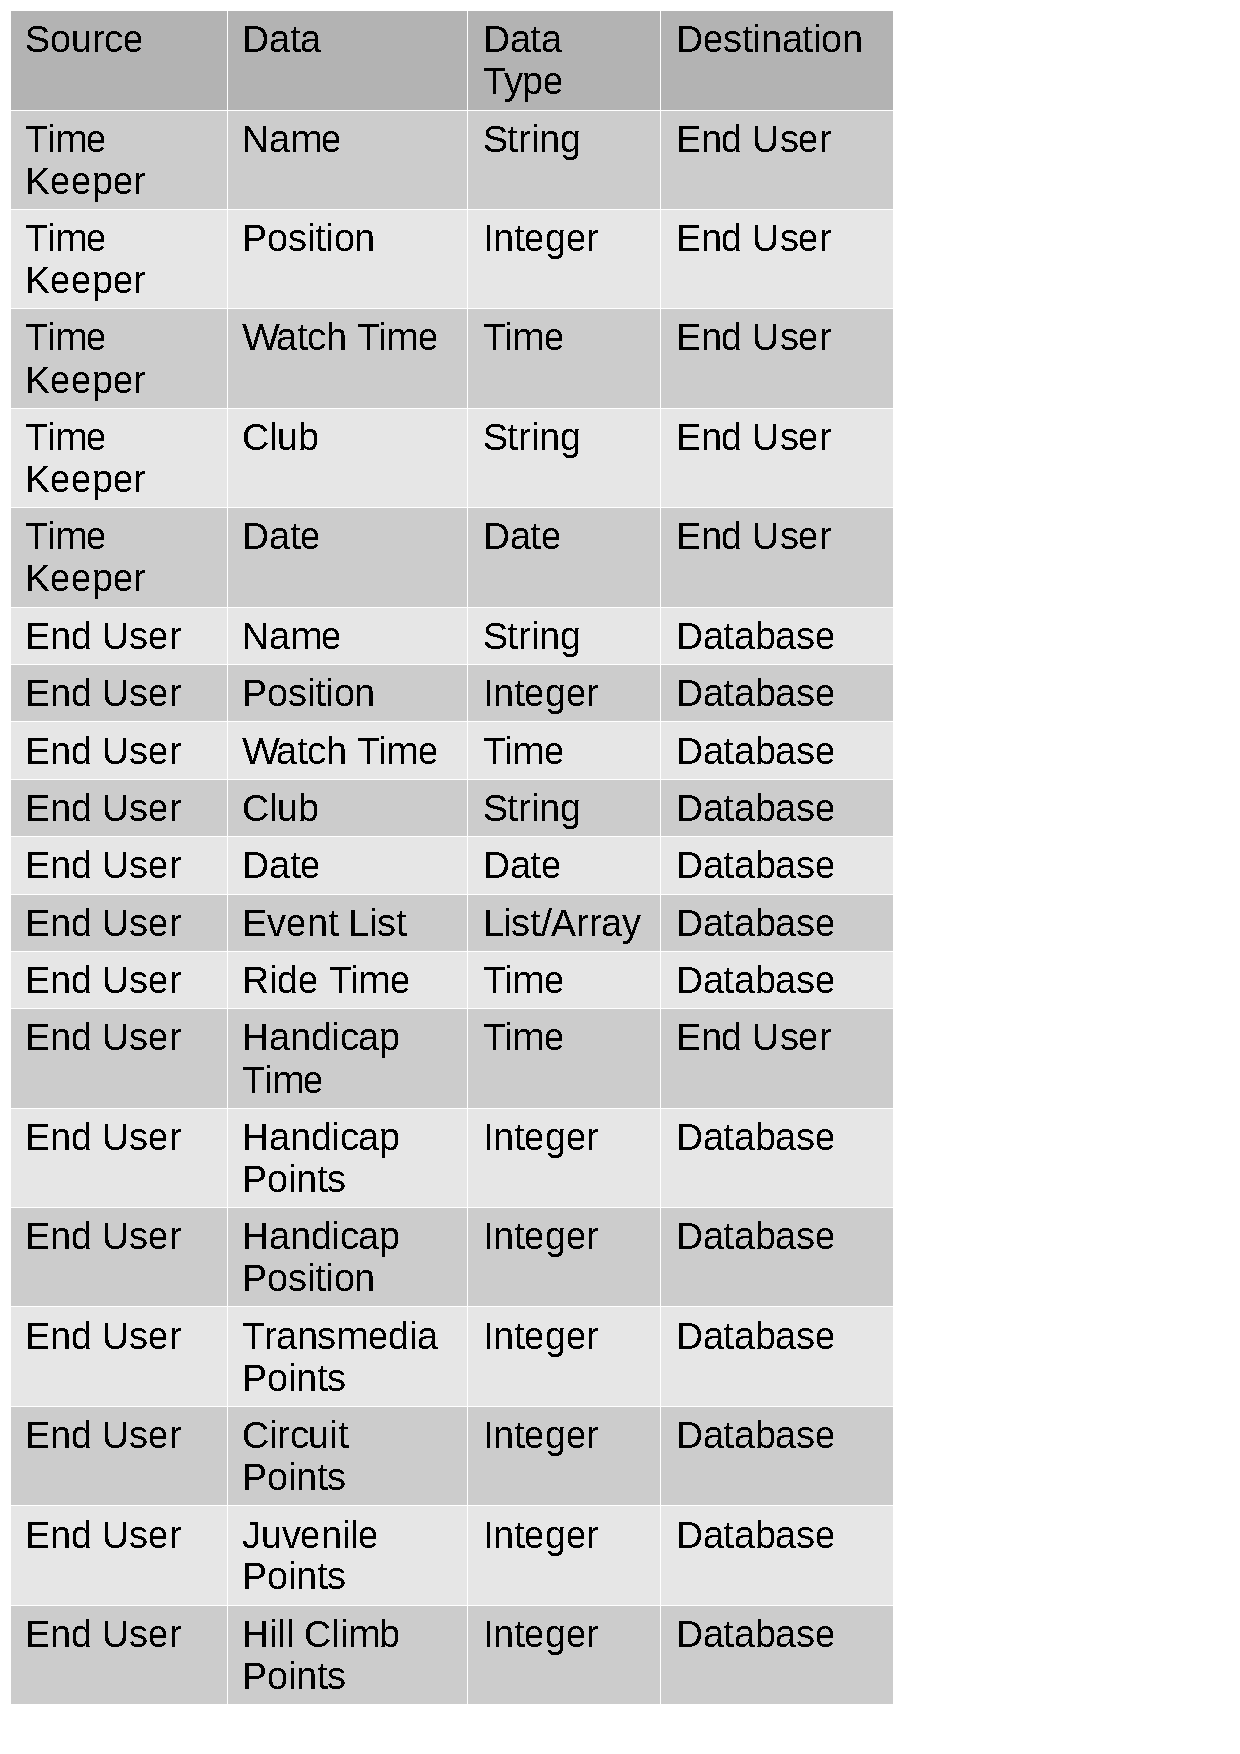
\includegraphics[width=\textwidth]{./DataSourcesPS.pdf}
	 \caption{Data sources and destinations of the proposed system}
\end{figure}

The data sources and destination of the proposed system are very similar to the current system as the project aims to automate the current system rather than change the current one.

\begin{tabular}{|l|l|l|l|}
\hline
SOURCE & DATA & DATA TYPE & DESTINATION  \\ \hline
Timekeeper & Name & String & End User  \\ \hline
Timekeeper & Position & Integer & End User  \\ \hline
Timekeeper & Watch Time & Time & End User  \\ \hline
Timekeeper & Club & String & End User  \\ \hline
Timekeeper & Date & Date& End User  \\ \hline
End User & Name & Sting & Database   \\ \hline
End User & Position & Integer & Database  \\ \hline
End User & Watch Time & Time & Database  \\ \hline
End User & Club & Sting & Database  \\ \hline
End User & Date & Date & Database  \\ \hline
End User & Event List & List/Array & Database  \\ \hline
End User & Ride Time & Time & Database  \\ \hline
End User & Handicap Time & Time & Database  \\ \hline
End User & Handicap Points & Integer & Database  \\ \hline
End User & handicap Position & Integer & Database  \\ \hline
End User & Transmedia Points & Integer & Database  \\ \hline
End User & Circuit Points & Integer & Database \\ \hline
End User & Juvenile Points & Integer & Database  \\ \hline
End User & Hill Climb Points & Integer & Database  \\ \hline
\end{tabular}
\subsection{The proposed system}


\subsubsection{Data flow diagram}

The data flow diagrams for the proposed system are nearly identical to the current system as there will be no change in the algorithms or the sources of data.
\begin{figure}[H]
	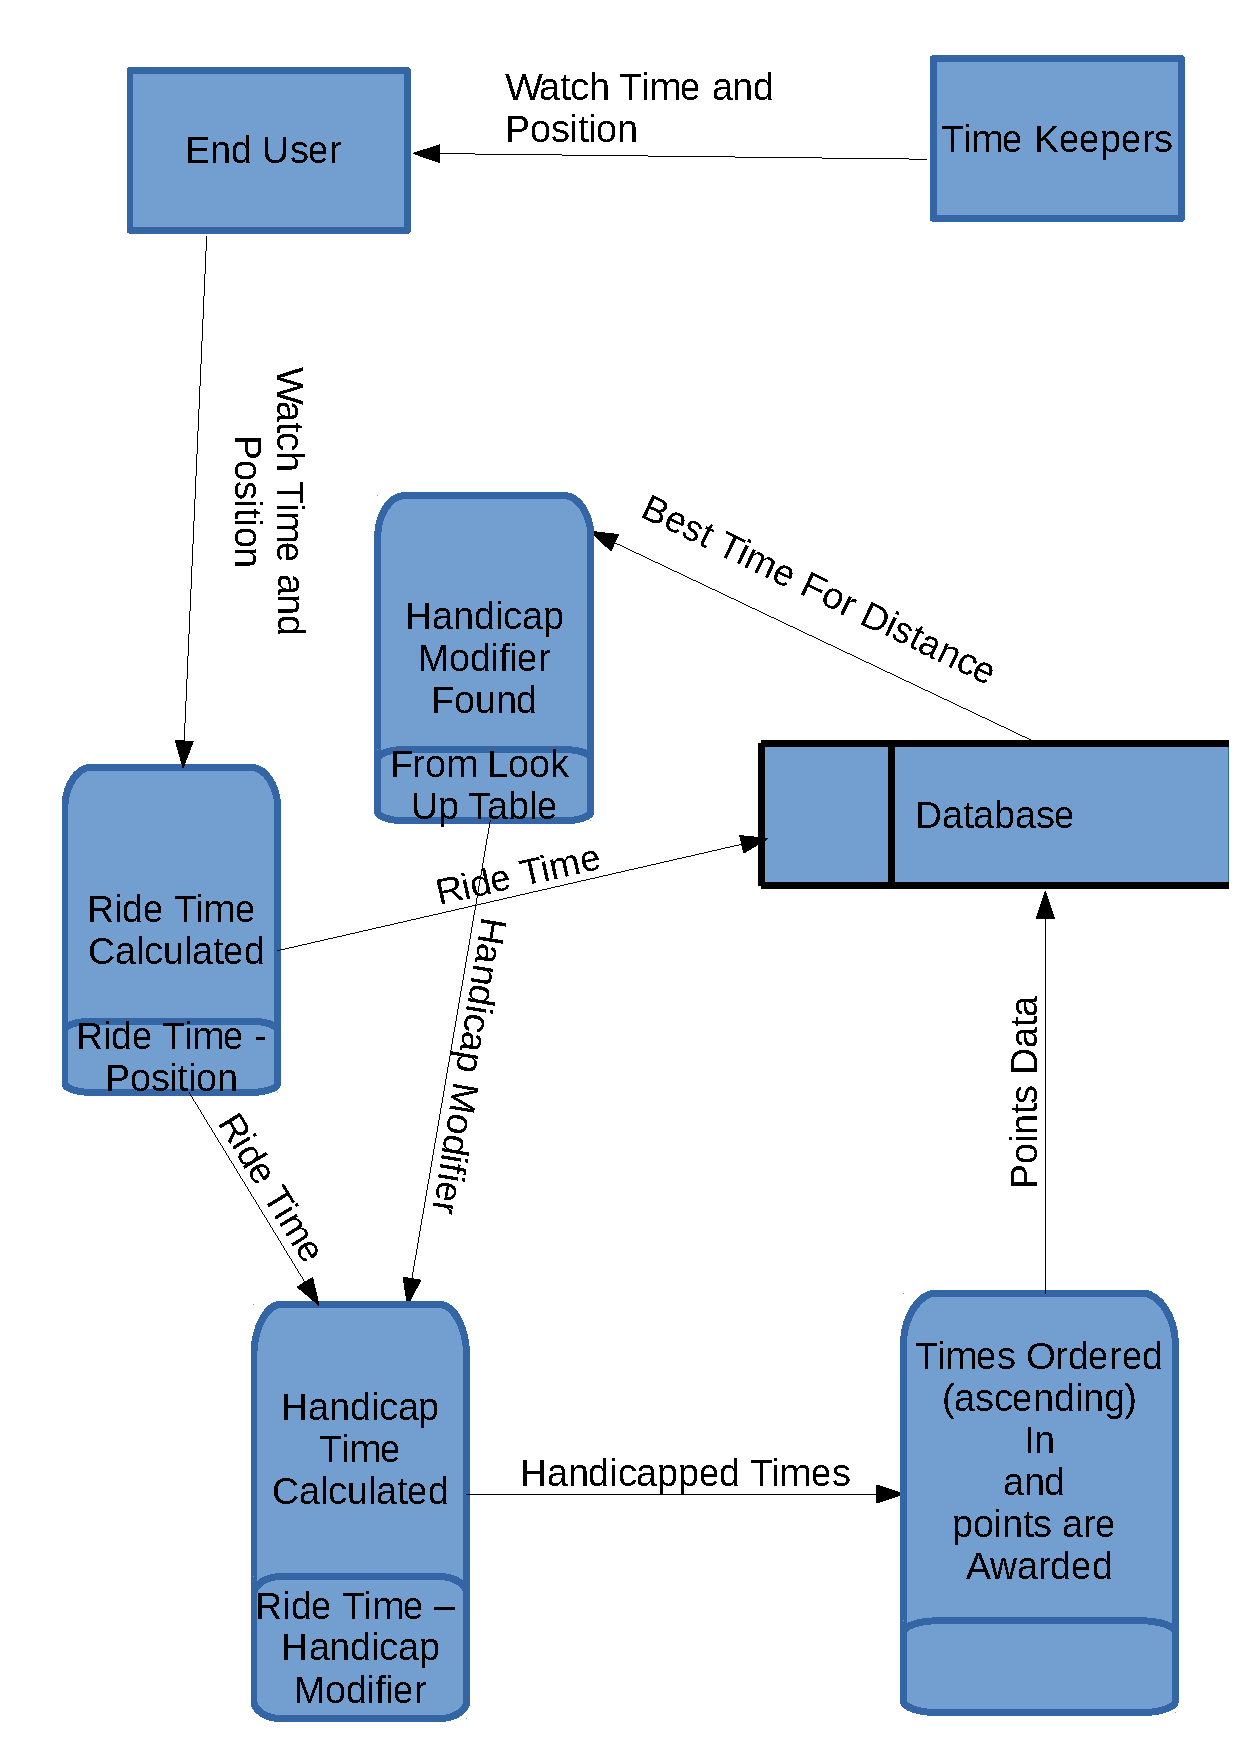
\includegraphics[width=\textwidth]{./DFDPS.pdf}
	 \caption{Data Flow Diagram for a Handicap event}
\end{figure}

\begin{figure}
	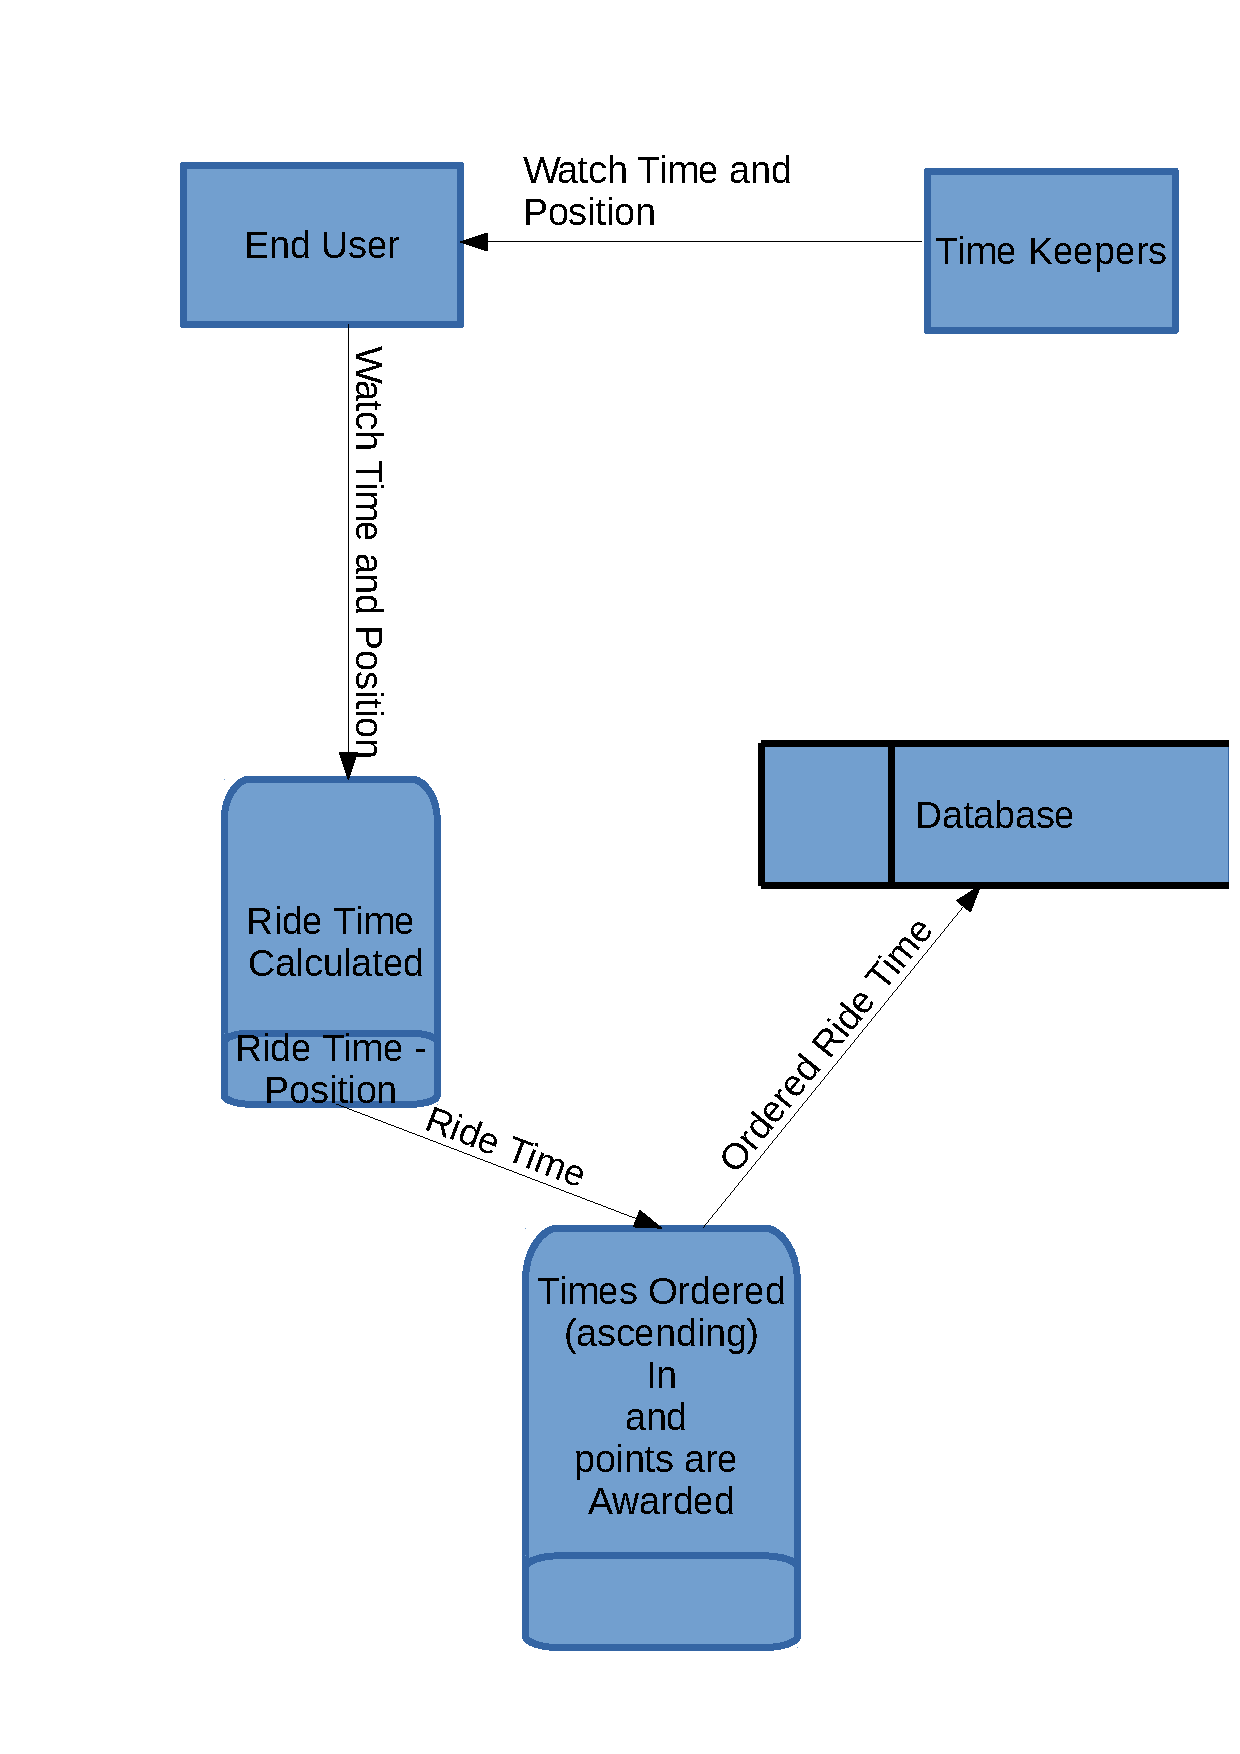
\includegraphics[width=\textwidth]{./Non-HandicapDFD-PS.pdf}
	\caption{Data flow diagram for a non-handicap event}
\end{figure}

The data flow diagrams are going to be identical for the proposed system as the aim of the project is to automate the current system rather than change the method that is used.


\subsubsection{Data dictionary}

\begin{figure}[H]
	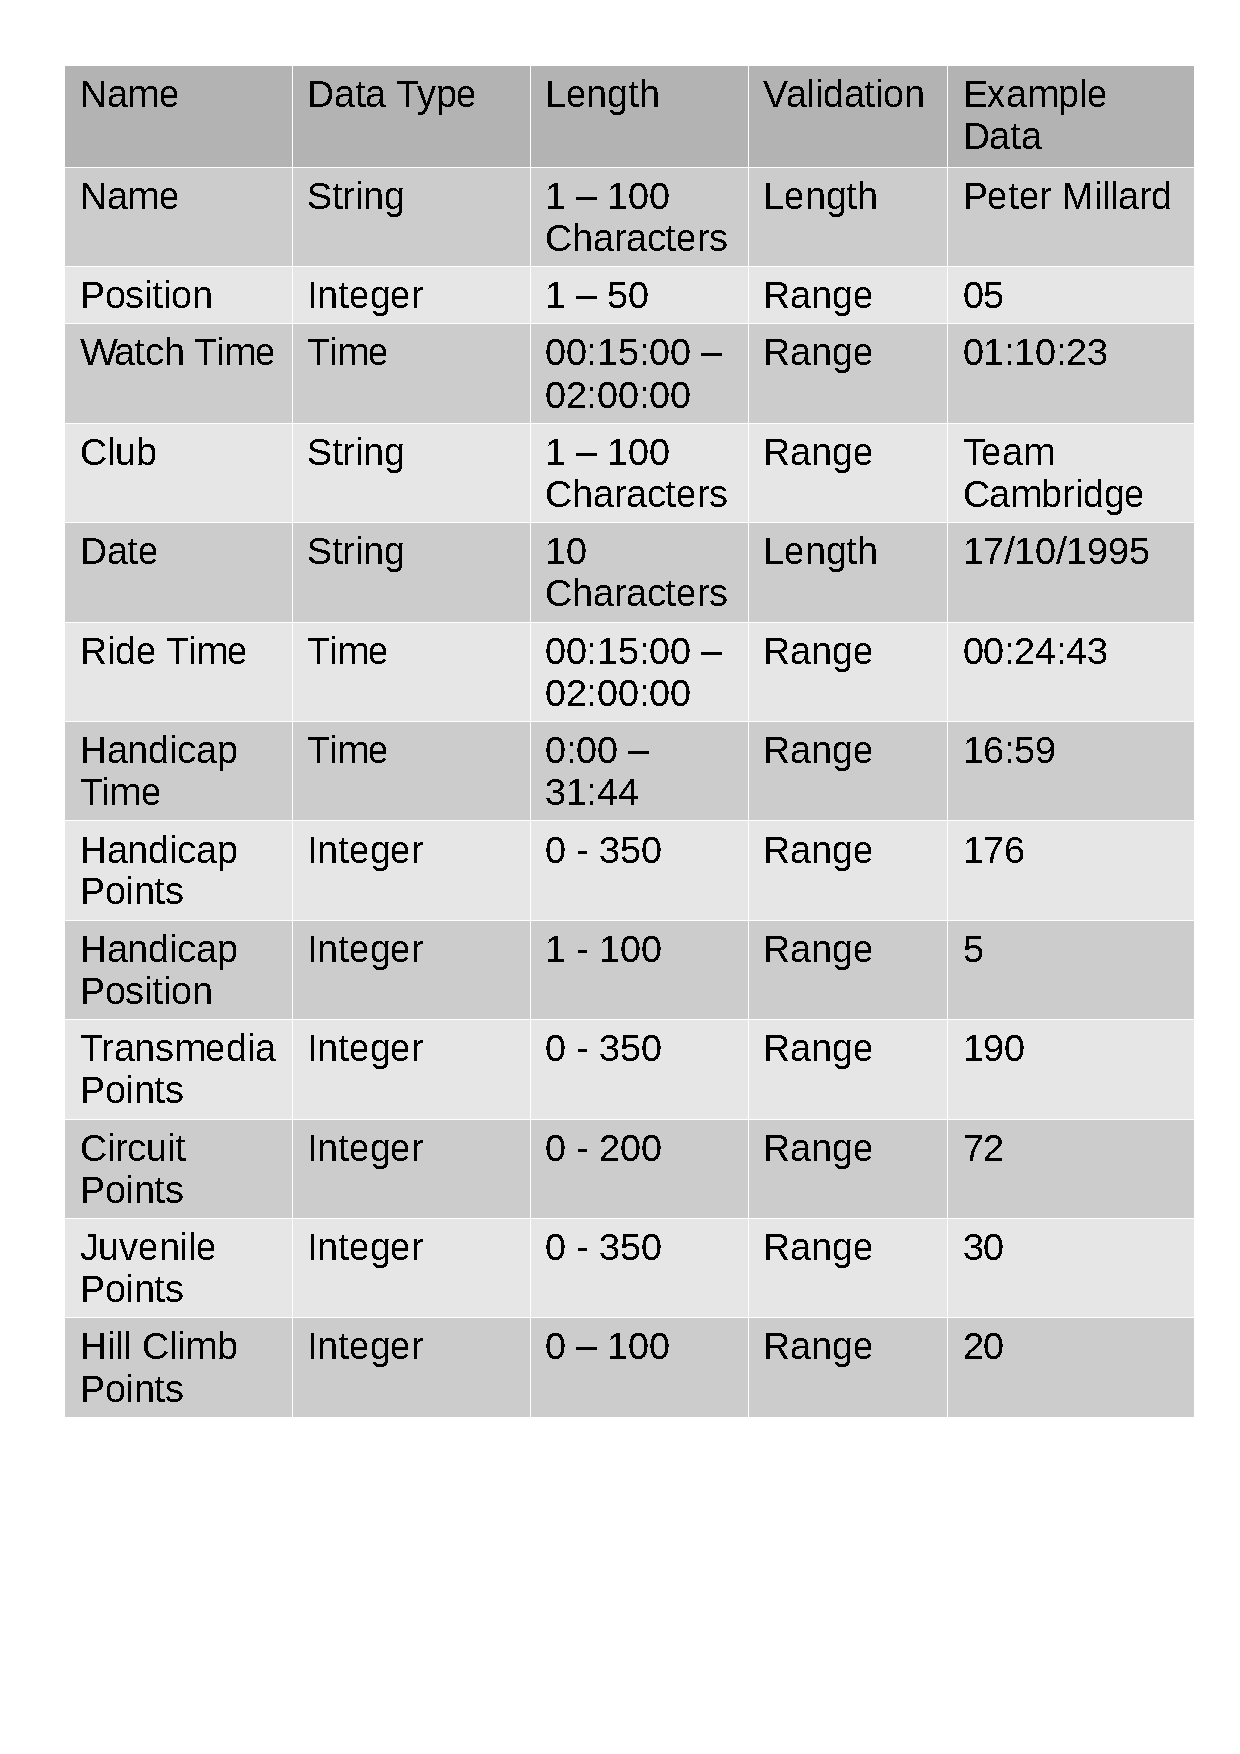
\includegraphics[width=\textwidth]{./DataDic.pdf}
	\caption{Dictionary of data}
\end{figure}


\begin{tabular}{|p{1.5cm}|p{1.5cm}|l|l|l|p{2.5cm}|}
	\hline
	NAME & DATA TYPE & LENGTH & VALIDATION & EXAMPLE DATA & APPROXIMATE SIZE \\ \hline
	Name & String & 1 - 100 Characters & Length & Peter Millard & 100 Bytes \\ \hline
	Position & Integer & 1 - 50 & Range & 05 & 4 Bytes \\ \hline
	Watch Time & Time & 00:15:00 - 02:00:00 & Range & 01:10:23 & 3 Bytes \\ \hline
	Club & String & 1 - 100 Characters & Range & Team Cambridge &  100 Bytes\\ \hline
	Date & date & DD/MM/YYYY & Length & 17/10/1995 & 3 Bytes \\ \hline
	Ride Time & Time & 00:15:00 - 02:00:00 & Range & 00:24:43 & 3 Bytes \\ \hline
	Handicap Time & Time & 0:00 - 31:44 & Range & 16:59 & 3 Bytes \\ \hline
	Handicap Points & Integer & 0 - 350 & Range & 176 & 4 Bytes \\ \hline
	Handicap Position & Integer & 1 -100 & Range & 5 & 4 Bytes \\ \hline
	Transmedia Points & Integer & 0- 350 & Range & 190& 4 Bytes \\ \hline
	Circuit Points & Integer & 0 - 200 & Range & 72 & 4 Bytes \\ \hline	
	Juvenile Points & Integer & 0 - 350 & Range & 30 & 4 Bytes \\ \hline
	Hill Climb Points & Integer & 0 - 100 & Range & 20 &  4 Bytes\\ \hline
\end{tabular}

\subsubsection{Volumetrics}
The current database contains around 7800 records, the size of this on disk is approximately 0.3 MB. This is made up from partial records from 1989 - 1996 and then complete records from 1996 - present.

If each record  contains a complete set of data in the data dictionary and there is a complete set of records from 1989 - present (including the missing records) this gives us 10,000 records over 25 years and we want the system to be used for another 25 years then 20,000 records is our estimate. 
 
The total amount of data for one record is 243 Bytes multiply this by the 20,000 estimate which gives an estimate of 4,860,000 Bytes or 4.86 Megabytes
\section{Objectives}

\subsection{General Objectives}
The General objectives of the project are:
\begin{itemize}
	\item To have a program that's easy enough for any member to upload the event results
	\item Clear and simple data entry form that any user can follow
	\item The user has to be able to follow the processes
	\item The Program needs to keep the minimal amount of data to keep the total amount of data in the database as low as possible
\end{itemize}

\subsection{Specific Objectives}
The specific Objectives of the project are:
\begin{itemize}
	\item Identify improvements to the current database
	\item Only retain essential data required for website users
	\item minimal data entry, so that the end user only has to input the name, watch time, club, age, Position, event date and event code
	\item The program needs to allow the user to edit the final data set, so any errors can be manually rectified
\end{itemize}

\subsection{Core Objectives}


The core objectives of the project are:
\begin{itemize}
	\item The program needs to be able to calculate times and apply the points and positions for Team Cambridge specific competitions
	\item The program needs to be able to upload the data to the Team Cambridge website
\end{itemize}
\subsection{Other Objectives}
Other objectives of the project are:
\begin{itemize}
	\item To retain the current results database
	\item If I have enough time, to have the database being run off Network Attached Storage
	\item If I have enough Time, to have a web interface that allows users to remotely access the database and upload results
\end{itemize}

\section{ER Diagrams and Descriptions}

\subsection{ER Diagram}

\begin{figure}[H]

	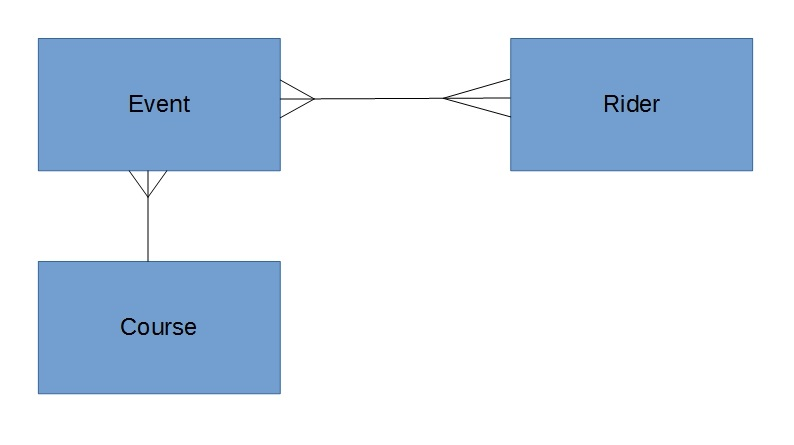
\includegraphics[width=\textwidth]{./ER.jpg}
	\caption{Entity relationship diagram of the system}
\end{figure}



\subsection{Entity Descriptions}
Event(\underline{EventID}, Date, \emph{CourseID}, Circuit Series, Handicap10, Handicap25, HillClimb, Transmedia, Juvenile)

Rider(\underline{RiderID}, Forename, Surname, Handicap10Points, CircuitPoints, TransmediaPoints, JuvenlePoints, Age)

Course(\underline{CourseID}, Distance, Type)

Record(\underline{RecordID}, \emph{RiderID},\emph{EventID}, RideTime, HandicapTime, RacePosition, Club)



\subsection{Entity Descriptions}
Event(\underline{EventID}, Date, \emph{CourseID}, \emph{RiderList*})

Rider(\underline{RiderID}, Forename, Surname, Handicap10Points, CircuitPoints, TransmediaPoints, JuvenlePoints, Age)

Course(\underline{CourseID}, Distance, Type)

RiderRecord(\underline{RRID}, \emph{RiderID}, RideTime, HandicapTime, Position, Club)

*List of 'RiderRecords'
\section{Object Analysis}

\subsection{Object Listing}
There will be 4 objects in the system:

\begin{enumerate}
    \item Events
    \item Course
    \item Riders

    \item RiderRecords

    \item Records
    \item TeamCambridgeRider

\end{enumerate}
\subsection{Relationship diagrams}

\subsection{Class definitions}
\begin{figure}[H]

	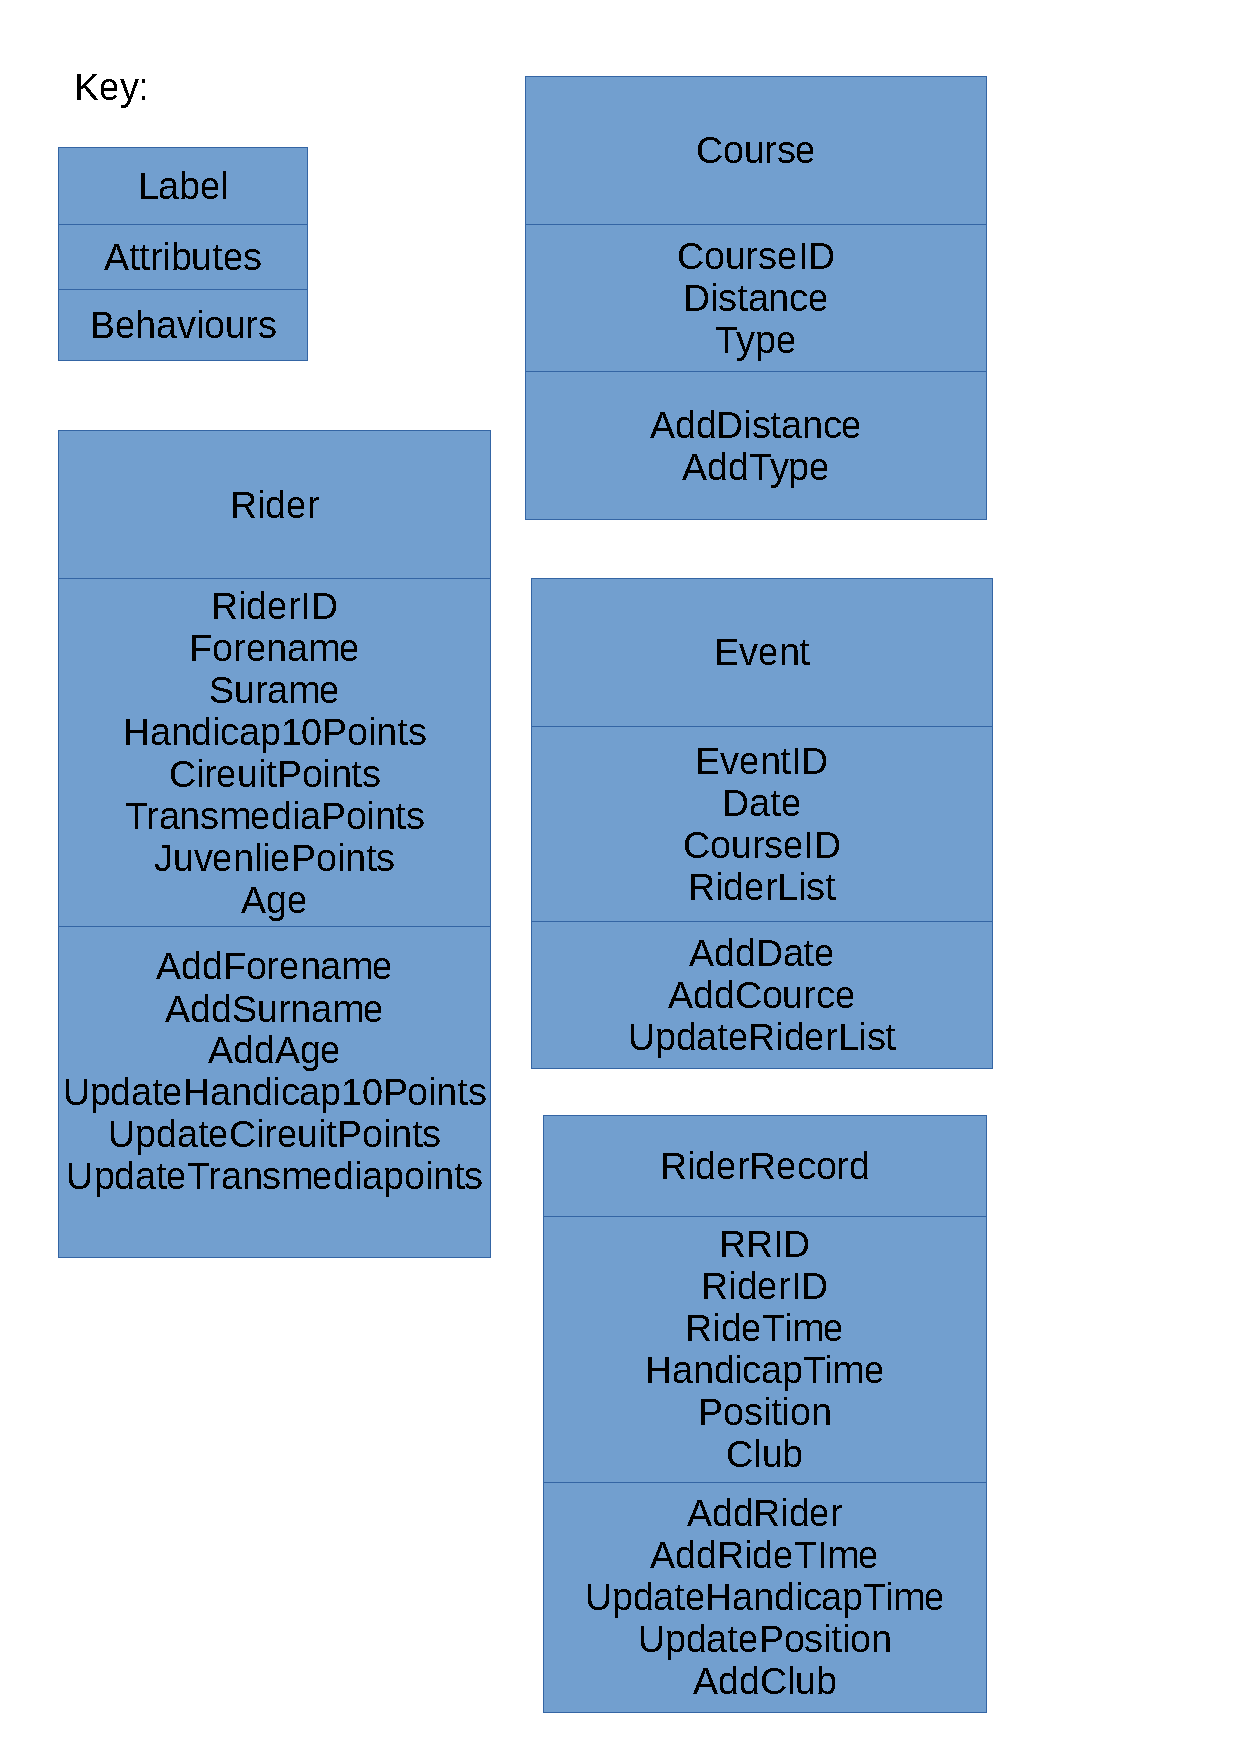
\includegraphics[width=\textwidth]{./Class.pdf}

	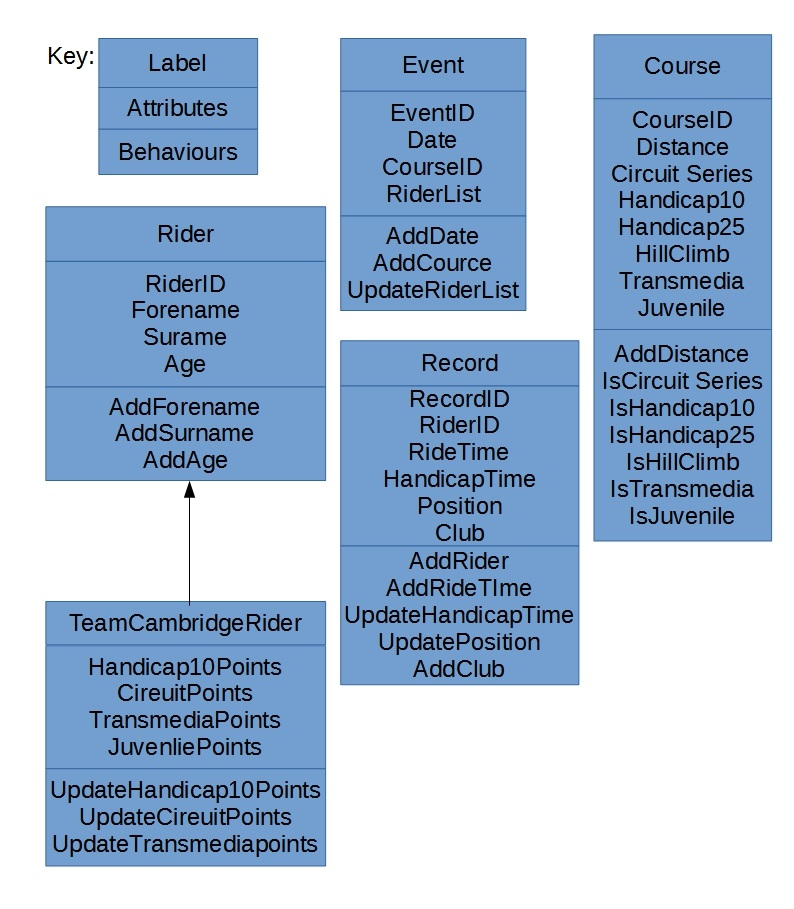
\includegraphics[width=\textwidth]{./Class.jpg}

	\caption{Class definitions of the system}
\end{figure}
\section{Other Abstractions and Graphs}
There are no other graphs that I need to include in this section.
\section{Constraints}

\subsection{Hardware}

The current system is run off an Acer laptop with the following system specification:

\begin{itemize}
\item OS: Windows Vista 32 Bit
\item CPU: Intel Pentium @ 2.16 GHz
\item GPU:Mobile Intel(R) 4 Series 
\item RAM: 3 GB
\item Storage: 144 GB HDD
\end{itemize}

This is going to be used as the minimum requirements as it should be representative of most members that will use this program will likely have similar or better hardware.

The system should be able to be run off any PC as the only hardware restriction that may affect the program in RAM. the existing system is being run on a Acer laptop with 4 GB of RAM and windows Vista 32 bit. This should be more than enough as the program will not be making large amounts of calculations that will require a high end CPU. As long as I manage variables correctly hardware will not be an issue.


The Client does not want their members to have to buy additional software to allow the program to work as the program will be used by multiple members. The only exception to this is that the Race Sectary has requested that I use the current database rather than crease a new one, however the Race Sectary will allow me to make modifications to the current database so I can improve it by normalization.

The Client does not want their members to have to buy additional software to allow the program to work as the program will be used by multiple members. This will not be an issue as I plan to create the program my self rather than using pre built software.
>>>>>>> branch 'master' of https://github.com/24697/COMP4Coursework.git
\subsection{Time}
<<<<<<< HEAD
The client has not set a deadline for the project so the only time restriction is those set by my teacher. However my client would prefer the project to be completed by the start of the next racing season.

The client has not set a deadline for the project so the only time restriction is those set by my teacher which is Friday 13th February 2015. However my client would prefer the project to be completed by the start of the next racing season, which will start in April 2015. This is likely contain the system heavily as that provides me with a short development period.

\subsection{User Knowledge}

The user has to be able to use the program without any knowledge of the current system, I will assume that any user is competent with a computer as they would have been trusted with the permissions associated with the database. If they were not trusted, then they would not be using the system.

The user has to be able to use the program without any knowledge of the existing system, I will assume that any user is competent with a computer as they would have been trusted with the permissions associated with the database. If they were not trusted, then they would not be using the system.

\subsection{Access restrictions}

The current database is controlled by permissions, as issued by the racing secretary. The client wishes to keep this system in place.

The current database is controlled by permissions, as issued by the Racing Secretary. The client wishes to keep this system in place.

\section{Limitations}

\subsection{Areas which will not be included in computerisation}
Data entry will be the only part of the system that can't be computerised. Data entry could be computerised by software that can scan forms and extract data from the form, however this would be too complicated to program.
\subsection{Areas considered for future computerisation}
Data Collection could be computerised by using sensor attached to the bikes that can be scanned when passing over the start/finish line to automatically time the riders. This would requer large amounts of research and development
\section{Solutions}

\subsection{Alternative solutions}

\subsection{Justification of chosen solution}
I have chosen to use a Python Desktop Application with a GUI.
